\documentclass[24pt]{beamer}

\usepackage[utf8]{inputenc} \usepackage{amsmath} \usepackage{amsfonts}
\usepackage{amssymb} \usepackage{booktabs} \usepackage{algpseudocodex}
\usepackage{xurl} \usepackage{multicol} \usepackage{dejavu} \usepackage{eurosym} \usepackage{listings}\usepackage{xcolor}
\usepackage{tabularx}

\lstset{
	language=Python,
	basicstyle=\ttfamily\small,
	keywordstyle=\color{purple},
	stringstyle=\color{blue},
	commentstyle=\color{gray},
	showstringspaces=false,
	showtabs=false,
	keepspaces=true,
	tabsize=4,
	columns=flexible
}

\usetheme{Antibes}

\usefonttheme{serif}
\setbeamerfont{caption}{size=\tiny} 
\graphicspath{{resources}}

\newcommand{\code}[1]{\texttt{#1}}

\title[LLM Optimization]{Creating and Deploying Production-Ready Agentic Systems}
\author{Dimitris Tsirmpas} \date{\today}
\institute{Athens University of Economics and Business \and Archimedes, Athena Research Center}

\begin{document}
    
\begin{frame}
    \titlepage
\end{frame}

\part{Autonomous LLM Agents}

\begin{frame}
   	\partpage
\end{frame}


\section{LLMs as System Components}

 \begin{frame}{Outline}
   	\tableofcontents[currentsection]
\end{frame}

\subsection{Inherent LLM limitations}

 \begin{frame}
   	\sectionpage
   	\subsectionpage
\end{frame}

\begin{frame}{Mathematics}
	\begin{block}{LLMs are terrible at math}
		\begin{itemize}
			\item Predict the most likely sequence of tokens, not the logically necessary derivation.
			\item Probabilistic nature $\rightarrow$ prone to hallucinations.
			\item Tokenization absolutely destroys numbers.
		\end{itemize}
	\end{block}
	
	\begin{alertblock}{}
		While OK for small numbers (they can memorize some patterns), they generally fail at larger ones.
	\end{alertblock}
\end{frame}

\begin{frame}{Word counting}
	\begin{figure}
		\centering
		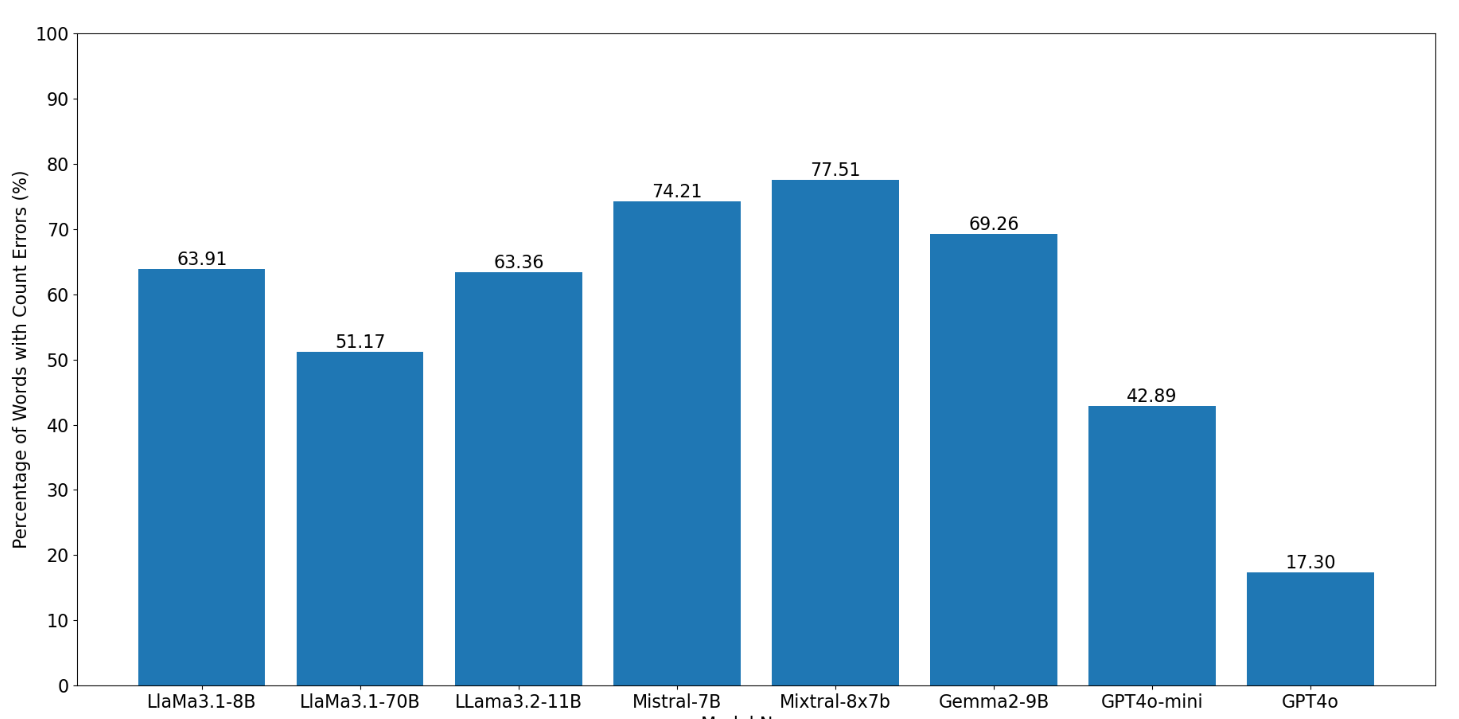
\includegraphics[width=\textwidth]{word-counting.png}
		\caption{Percentage of words with errors on when counting letters for the different models \url{https://arxiv.org/html/2412.18626v1}.}
	\end{figure}
\end{frame}

\begin{frame}[fragile]{Character counting}
   \begin{exampleblock}{Example}
\begin{lstlisting}
model.prompt("How many 'r's are in 'carr'?")
>>> "There is one 'r' in 'carr'".
\end{lstlisting}
	\end{exampleblock}
		
	\begin{block}{Indicative explanation}
		\begin{itemize}
			\item The model can not find the word ``carr'' in its knowledge base.
			\item But it knows the word ``car'' and the fact that ``carr'' and ``car'' are highly correlated.
			\item ``car'' has one ``r'', therefore this is the answer.
		\end{itemize}
	\end{block}
\end{frame}

\begin{frame}{Deductive reasoning}
	\begin{figure}
		\centering
		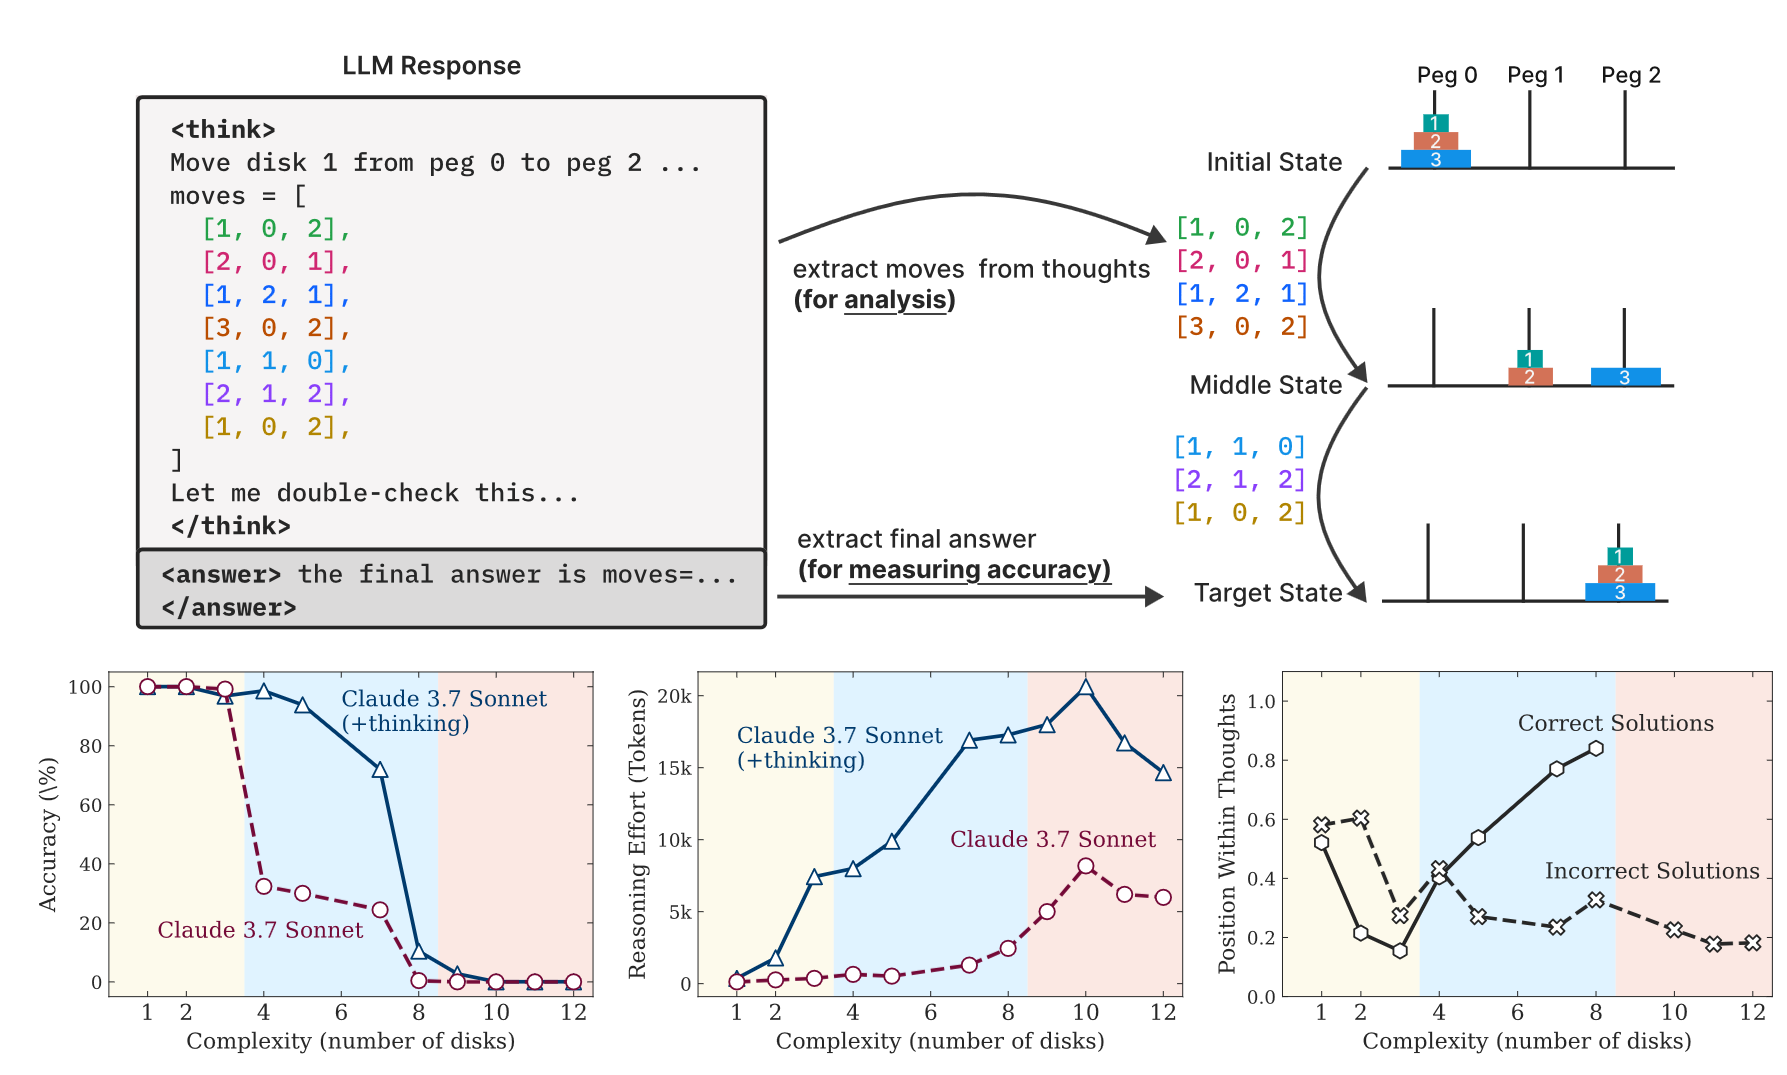
\includegraphics[width=\textwidth]{hanoi.png}
		\caption{Percentage of words with errors on when counting letters for the different models \url{https://arxiv.org/html/2412.18626v1}.}
	\end{figure}
	\note{Explain the problem of the towers of hanoi. Then, how this is represented through text. Then, how LLMs fail at it. Then, why LLMs fail at it.}
\end{frame}

\begin{frame}{General Limitations}
	\begin{alertblock}{LLMs cannot:}
		\begin{itemize}
			\item Think.
			\item Behave.
			\item Deduct.
		\end{itemize}
	\end{alertblock}
	
	\begin{block}{Why?}
		\begin{itemize}
			\item LLMs are generally \alert{excellent stochastic parrots}. Their \alert{next-word-prediction} nature prevents them from understanding the world and its mechanisms.
			\item Finetuning, reasoning and in-context learning alleviate, but do not bypass this restriction.
		\end{itemize}
		\note{Debate on whether LLMs are excellent Type I or very poor Type II systems. Also tie-in with debate around ML statistical field and symbolic AI.}
	\end{block}
\end{frame}

\begin{frame}{A Note on Benchmarks}
	\begin{columns}
		\begin{column}{0.5\textwidth}
			\begin{figure}
				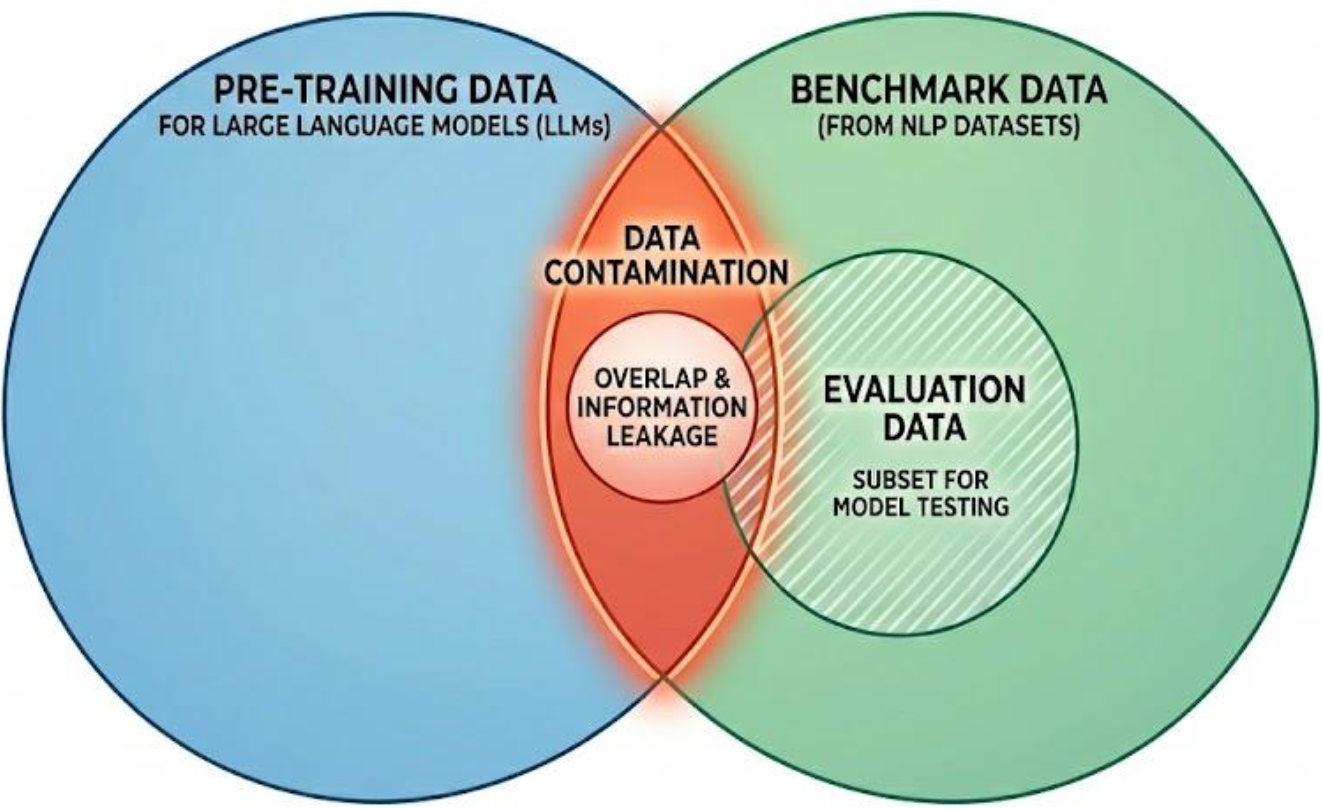
\includegraphics[width=\textwidth]{contamination.png}
				\caption{Credit to Electra Maria Papadopoulou---generated with Gemini.}
			\end{figure}
		\end{column}
		\begin{column}{0.5\textwidth}
			\begin{block}{Data Contamination}
				\begin{itemize}
					\item Evaluation data appears in training.
					\item Web-scraping may include datasets used as
					training, validation, or
					benchmarks, unknowingly inflating reported performance.
					\item Sometimes on purpose (``benchmaxxing'').
				\end{itemize}
			\end{block}
		\end{column}
   	\end{columns}
\end{frame}

\begin{frame}{A Note on Benchmarks}
	\begin{columns}
		\begin{column}{0.5\textwidth}
			\begin{figure}
				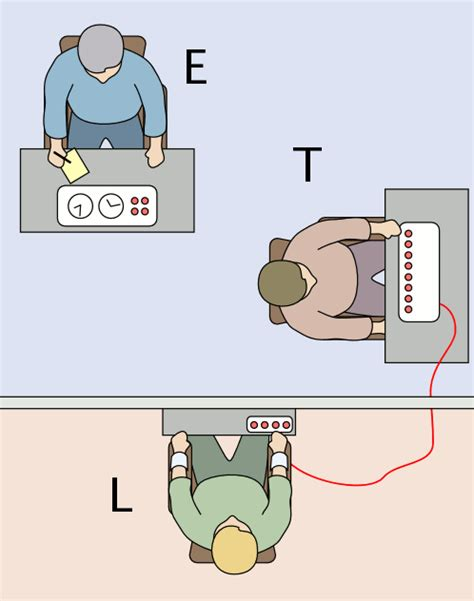
\includegraphics[width=\textwidth]{milgram.jpg}
				\caption{Credit to Electra Maria Papadopoulou---generated with Gemini.}
			\end{figure}
		\end{column}
		
		\begin{column}{0.5\textwidth}
		\begin{exampleblock}{Behavior replication}
			\begin{itemize}
				\item LLMs replicate the Milgram study.
				\item Emergent social property!
				\item ...or is it that the LLMs already know the results of the study?
				\item Perhaps, they implicitly follow what they know humans do.
			\end{itemize}
		\end{exampleblock}
	\end{column}
	\end{columns}
\end{frame}

\begin{frame}{A Note on Benchmarks}
	\begin{block}{Benchmaxxing}
		Optimizing a LLM's performance primarily for high scores on public \alert{leaderboards} and \alert{benchmarks}, rather than practical, and reliable real-world capability. 
	\end{block}
	
	\begin{block}{How?}
		\begin{itemize}
			\item Training Data Contamination.
			\item Format Overfitting.\note{A model fine-tuned heavily on the specific format of the benchmark learns to exploit statistical quirks—such as predicting that the correct answer is disproportionately in position 'C', or applying specific elimination heuristics—rather than improving its underlying knowledge or reasoning ability. }
			\item Checkpoint Cherry-Picking.
			\item Prompt Engineering.\note{A lab can tune the evaluation ""harness""—the system prompts, the chain-of-thought templates, and the answer extraction methods—to maximize the score on a specific benchmark, potentially adding several percentage points without changing the model's actual underlying weights.}
		\end{itemize}
	\end{block}
\end{frame}


\subsection{When to use LLMs?}

\begin{frame}
	\sectionpage
	\subsectionpage
\end{frame}

\begin{frame}{LLMs are not just task-specific tools}
	\begin{itemize}
		\item So far, we have used LLMs as specialized tools for specific tasks.
		\item While useful, these tasks can generally be accomplished by \alert{simpler} and more \alert{scalable} models (with some performance loss).
		\item Where LLMs differ, is that they are \alert{autonomous}, which allows for \alert{previously impossible} use-cases.
	\end{itemize}
\end{frame}

\begin{frame}{When you are holding a hammer...}
	\begin{itemize}
		\item Suppose you are given the following task, with appropriate resources from management.
	\end{itemize}
	\begin{exampleblock}{Use case}
		Find all reviews that concern competitors of our product, and tell us what percentage of them mention it.
	\end{exampleblock}
\end{frame}

\begin{frame}{When you are holding a hammer...}   	
	\begin{block}{Our problem could be decomposed in three parts}  		
		\begin{enumerate}
			\item Discovery: Find pages containing reviews.
			\item Filtering: Find the HTML sections containing the reviews.
			\item Analysis: Find which reviews reference the product.
		\end{enumerate}
	\end{block}
   	
	\begin{alertblock}{}
		Which of these must necessarily be solved with LLMs? Which can be solved with traditional ways? What trade-offs are we making in the latter case?
	\end{alertblock}
\end{frame}

\begin{frame}{... you treat everything as if it were a nail}
	\begin{block}{The easy solution}
		We instruct an LLM to retrieve reviews via RAG. We isolate the reviews using prompting, then instruct the LLM to find whether our product is mentioned.
	\end{block}
   	
	\begin{exampleblock}{Result}
		Code is deployed \alert{within the day}. Management is billed \alert{50,000\euro} in a week.
	\end{exampleblock}
\end{frame}

\begin{frame}{But maybe we can do better}
	\begin{block}{The system solution}
		We use a traditional scrapper to find relevant reviews. For each page, we instruct the LLM to extract the reviews. We then run \code{reviews.str.contains(product\_name).sum()}.
	\end{block}
	
	\begin{exampleblock}{Result}
		Code is deployed within \alert{two days}. Management is billed \alert{20\euro} in a week.
	\end{exampleblock}
\end{frame}

\begin{frame}{Summing up}
	\begin{block}{LLMs as system components}
		\begin{itemize}
			\item Ordinary tasks that are trivial to humans or through programming may be exceptionally hard for LLMs.
			\item This fact motivates us to combine them with standard tools instead of relying on them for everything.
			\item Generally, LLMs should be thought of as functions which can adapt to the input.
		\end{itemize}
	\end{block}
\end{frame}

\section{Tool-Based Reasoning using ReAct}

\begin{frame}{Outline}
   	\tableofcontents[currentsection]
\end{frame}

\subsection{Thought, Action, Observation}

\begin{frame}
	\sectionpage
	\subsectionpage
\end{frame}

\begin{frame}[fragile]{Tool-Calling}
	\begin{exampleblock}{Tool example}
		
\begin{lstlisting}
from smolagents import tool

@tool
def calculator(expr: str) -> float:
    """
    Evaluate a basic arithmetic expression.
    Args:
    expr: The math expression to evaluate, such as 
    "2 + 3 * (4 / 2)".
    """
    return eval(expr, {"__builtins__": None}, {})
\end{lstlisting}
	
   \end{exampleblock}
\end{frame}

\begin{frame}{What is ReAct?}
	\begin{figure}
		\includegraphics[width=0.8\textwidth]{ReAct-definition.png}
		\caption{\url{https://arxiv.org/abs/2210.03629}}
	\end{figure}
	
	\begin{definition}
		\textbf{ReAct}:
		A technique that interleaves reasoning steps (``Thought'') with Actions and Observations to guide an LLM through planning and tool use.\note{No standard definition}
	\end{definition}
\end{frame}
    
\begin{frame}[fragile]
	\begin{exampleblock}{Tool calling example}
\begin{lstlisting}
{
    "tool_calls": [
    {
        "id": "calc1",
        "function": {
            "name": "calculate",
            "arguments": {
                "command": "calculator(
                '2 + 3 * (4 / 2)'
                )"
            }
        }
    }
    ]
}

>>> 8
\end{lstlisting}
	\end{exampleblock}
\end{frame}

\begin{frame}[fragile]
	\begin{exampleblock}{Tool calling chaining example}
		\begin{lstlisting}
"tool_calls": [
     {
        "id": "stock_call_1",
        "function": {
            "name": "get_stock_price",
            "arguments": {
                "ticker": "TSLA"
            }
      }
     },
    {
        "id": "news_call_2",
        "function": {
            "name": "fetch_news_summary",
            "arguments": {
                "ticker": "TSLA"
    [...]
		\end{lstlisting}
	\end{exampleblock}
\end{frame}
	  
\begin{frame}{High-level Concept}
	\begin{columns}
    		\begin{column}{0.6\textwidth}
    			\begin{figure}
    				\includegraphics[width=\textwidth]{ReAct-example3.png}
    				\caption{\url{https://arxiv.org/abs/2210.03629}}
    			\end{figure}
    		\end{column}
    		\begin{column}{0.4\textwidth}
    			\begin{block}{ReAct loop}
    					\begin{itemize}
    					\item Create a plan.
    					\item Identify action using reasoning (CoT).
    					\item Take action.
    					\item Observe result and update plan.
    				\end{itemize}
    			\end{block}
    		\end{column}
    	\end{columns}
\end{frame}

\begin{frame}{Early examples}
	\begin{columns}
		\begin{column}{0.5\textwidth}
				\begin{figure}
    				\includegraphics[width=\textwidth]{ReAct-example1.png}
    				\caption{\url{https://rdi.berkeley.edu/llm-agents/f24}}
    			\end{figure}
		\end{column}
		
		\begin{column}{0.5\textwidth}
			\begin{figure}
				\includegraphics[width=\textwidth]{ReAct-example2.png}
				\caption{\url{https://rdi.berkeley.edu/llm-agents/f24}}
			\end{figure}
		\end{column}
	\end{columns}
\end{frame}

\begin{frame}{Failure Modes Persist}
	\begin{figure}
		
\includegraphics[width=\textwidth]{react-failure.png}
		\caption{\url{https://x.com/i/status/2072864322536222875}}
	\end{figure}
	
	\begin{alertblock}{Do not blindly trust the system}
		LLMs can still hallucinate, even when reasoning and using tools.
	\end{alertblock}
\end{frame}


\subsection{Standardization}

\begin{frame}
	\sectionpage
	\subsectionpage
\end{frame}

\begin{frame}{Agency levels}
	\begin{figure}
		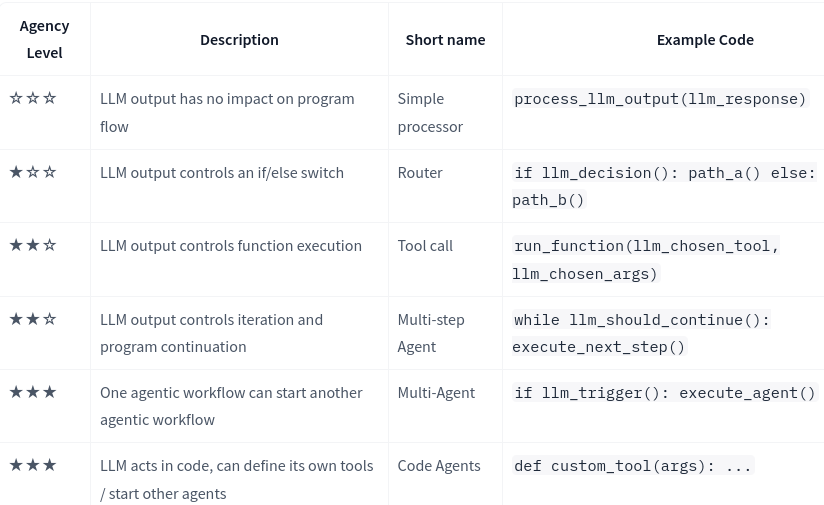
\includegraphics[width=0.9\textwidth]{agent-levels.png}
		\caption{\url{https://huggingface.co/docs/smolagents/en/conceptual_guides/intro_agents}}
	\end{figure}
\end{frame}

\begin{frame}{MCP: What is it?}
	\begin{columns}
		\begin{column}{0.5\textwidth}
			\begin{figure}
				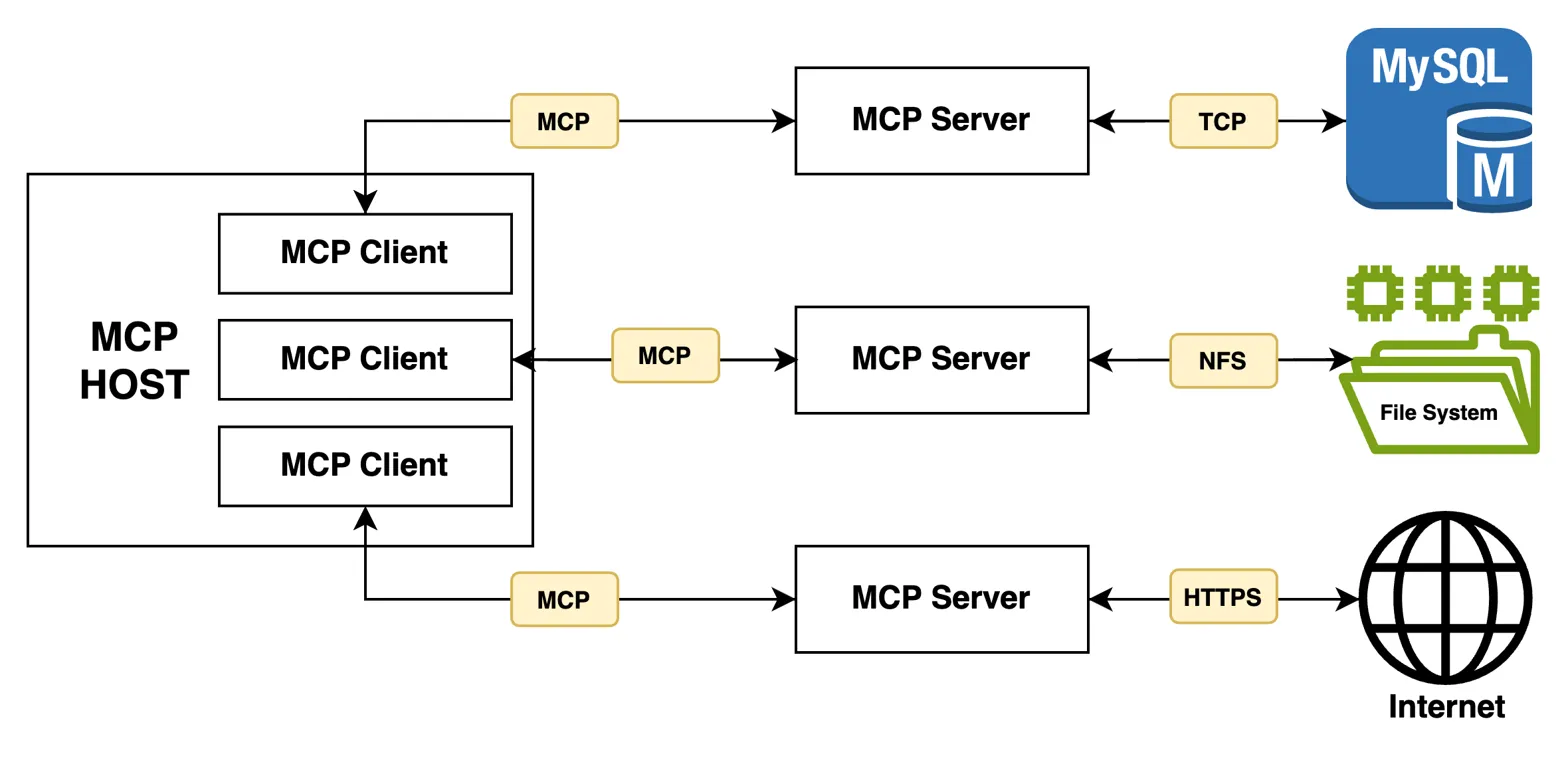
\includegraphics[width=\textwidth]{mcp.png}
				\caption{\url{https://velog.io}}
			\end{figure}
		\end{column}
		\begin{column}{0.5\textwidth}
			\only<1>{
				\begin{definition}[MCP]
					Model Context Protocol is a standardized framework that connects LLMs with external tools, APIs, and live data sources.
				\end{definition}
			}
			\only<2>{
				\begin{block}{Components}
					\begin{itemize}
						\item \textbf{MCP Server}: Backend executing standardized API calls.
						\item \textbf{MCP Client}: Translates LLM command to the MCP server.
						\item \textbf{MCP Host}: The LLM and UI.
					\end{itemize}
				\end{block}
			}
		\end{column}
	\end{columns}
\end{frame}

 \begin{frame}{MCP: Real-Use Example}
	\begin{figure}
		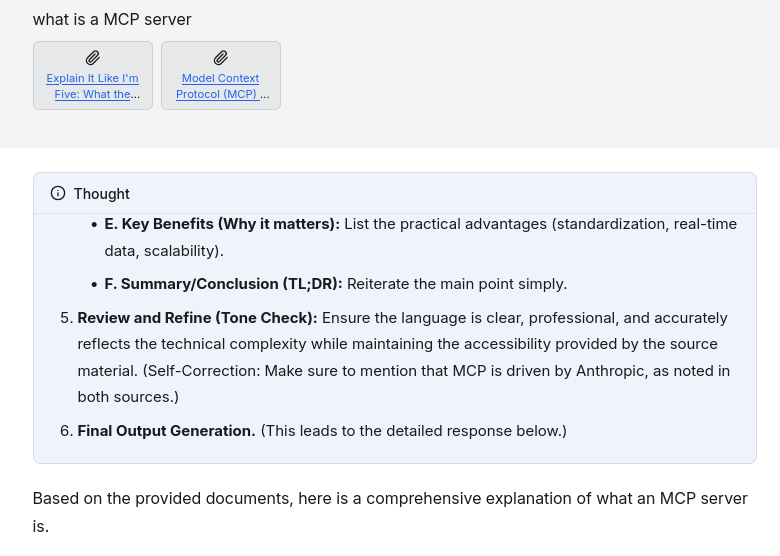
\includegraphics[width=0.6\textwidth]{mcp-ui.png}
		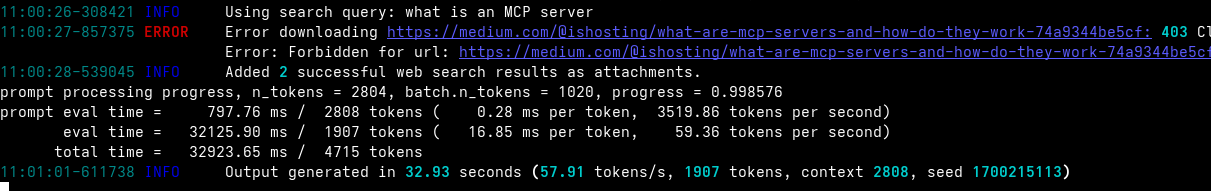
\includegraphics[width=\textwidth]{mcp-logs.png}
	\end{figure}
\end{frame}

\begin{frame}{MCP: Internals}
	\begin{columns}
		\begin{column}{0.5\textwidth}
			\begin{figure}
				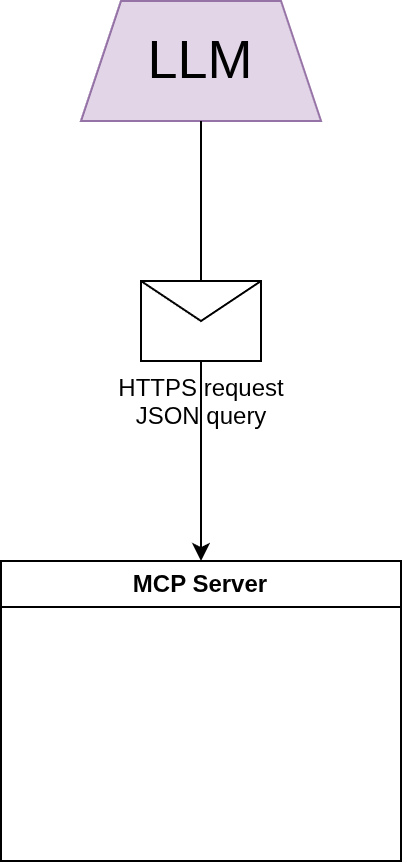
\includegraphics[height=0.8\textheight]{mcp-process1.png}
				\caption{\url{https://velog.io}}
			\end{figure}
		\end{column}
		\begin{column}{0.5\textwidth}
			\begin{itemize}
				\item The \alert{MCP Client} sends a JSON query.
				\item Query wrapped in a HTTPS request for validation and security.
			\end{itemize}
		\end{column}
	\end{columns}
\end{frame}

\begin{frame}{MCP: Internals}
	\begin{columns}
		\begin{column}{0.5\textwidth}
			\begin{figure}
				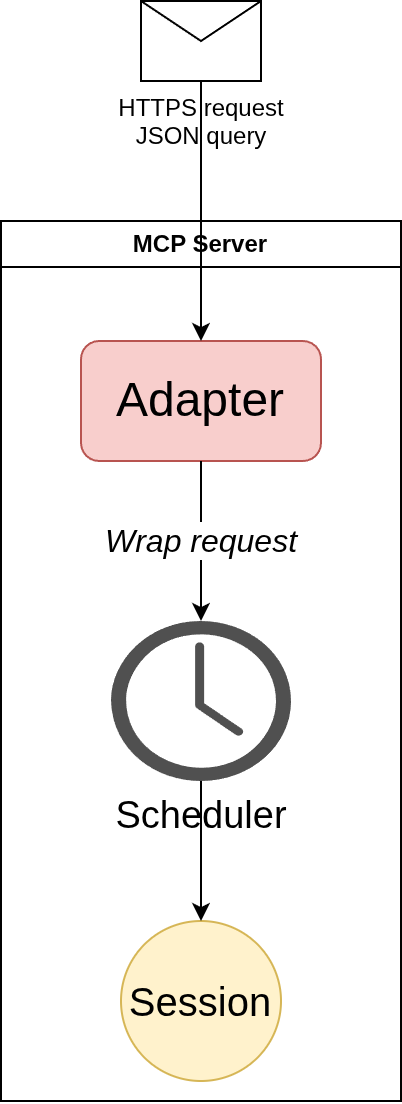
\includegraphics[height=0.8\textheight]{mcp-process2.png}
				\caption{\url{https://velog.io}}
			\end{figure}
		\end{column}
		\begin{column}{0.5\textwidth}
			\begin{itemize}
				\item The \alert{Adapter} receives the request.
				\item Attaches metadata (id, length etc.).
				\item Forwards the message to the \alert{Scheduler} which creates a session for the user.
				\item Enables concurrent requests by multiple users.
			\end{itemize}
		\end{column}
	\end{columns}
\end{frame}

\begin{frame}{MCP: Internals}
	\begin{columns}
		\begin{column}{0.5\textwidth}
			\begin{figure}
				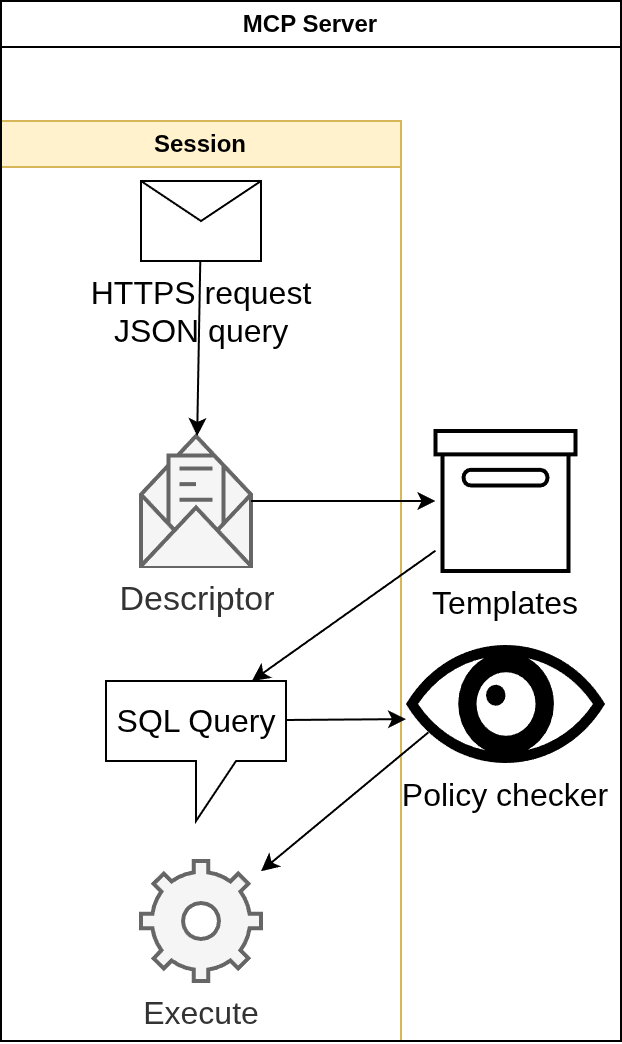
\includegraphics[height=0.8\textheight]{mcp-process3.png}
				\caption{\url{https://velog.io}}
			\end{figure}
		\end{column}
		\begin{column}{0.5\textwidth}
			\begin{itemize}
				\item Adapter's message contains a pointer to an \alert{existing template} (e.g., \texttt{customer.balance}).
				\item Retrieve standardized template (e.g., \texttt{SELECT balance FROM Accounts WHERE ...})
				\item Ensure that query has \alert{necessary permissions} (in this case, \texttt{READ} access).
			\end{itemize}
		\end{column}
	\end{columns}
\end{frame}

\begin{frame}{MCP: Internals}
	\begin{columns}
		\begin{column}{0.5\textwidth}
			\begin{figure}
				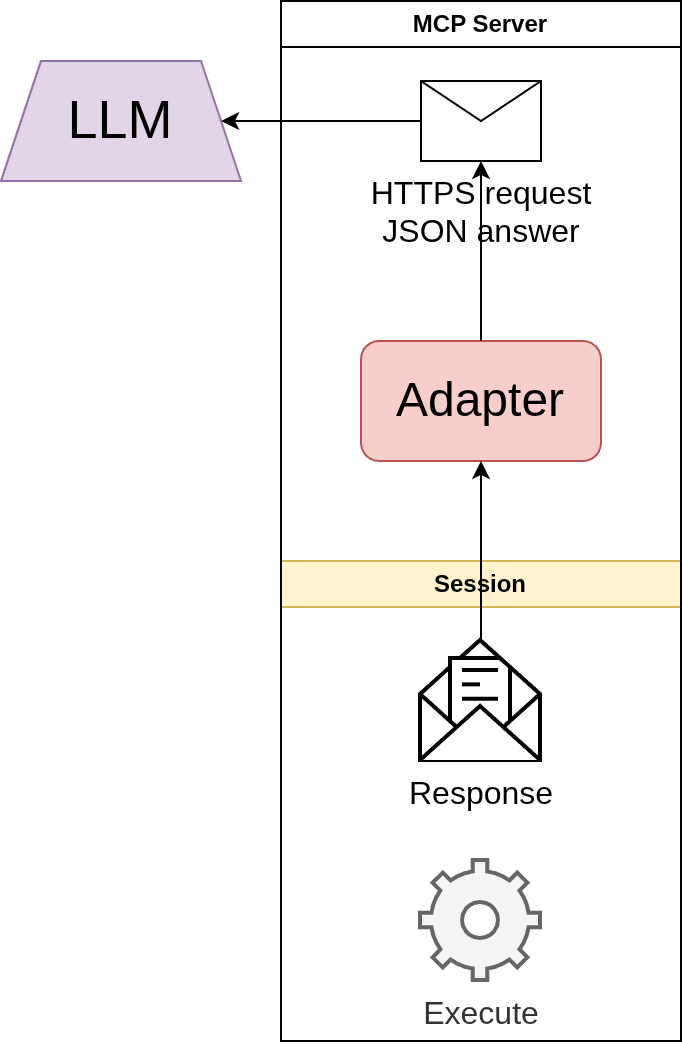
\includegraphics[height=0.8\textheight]{mcp-process4.png}
				\caption{\url{https://velog.io}}
			\end{figure}
		\end{column}
		\begin{column}{0.5\textwidth}
			\begin{itemize}
				\item Execute query with \alert{limited permissions} and \alert{tag} it (e.g., \texttt{READ} label) in case of further processing in the server.
				\item Adapter unpacks response and \alert{re-packages} it into a JSON object inside an HTTPS response.
			\end{itemize}
		\end{column}
	\end{columns}
\end{frame}

\begin{frame}{Summing up}
	\begin{block}{ReACT}
		\item The ReACT methodology was developed to allow autonomous use of tools by LLMs.
		\item This methodology combines a sandbox environment with standard and CoT prompting.
		\item Further standardization led to LLM agents with increasing autonomy as well as dedicated software architectures.
		\item The MCP architecture is the go-to modern solution for LLM tool use.
	\end{block}
\end{frame}


\section{Agent-to-Agent Interaction}

\subsection{Single-Agent vs. Multi-Agent}

\begin{frame}{Outline}
	\tableofcontents[currentsection]
\end{frame}

\subsection{Orchestrating Interaction}

\subsection{What do we actually need?}

\begin{frame}{Summing up}
	\begin{block}{Agent-to-Agent Interaction}
		\item We must select 
	\end{block}
\end{frame}

\part{Cost, Scalability, Accountability}

\begin{frame}
	\partpage
\end{frame}


\section{Opex vs capex in LLM systems}

\begin{frame}{What we will be talking about}
   	\tableofcontents
\end{frame}


\subsection{Local vs. Cloud Models}

\begin{frame}{Outline}
	\tableofcontents[currentsection]
\end{frame}

\begin{frame}{Different Cost Profiles}
	\begin{table}[ht]
		\centering
		\begin{tabularx}{\textwidth}{lXX}
			\toprule
			& \textbf{OpEx} & \textbf{CapEx} \\
			\midrule
			Constraints & Volume & Capabilities \\
			Funding & Continuous & Upfront \\
			Consumption & Immediate\note{electricity/API} & Depreciation \\
			\midrule
			Local Model & Low & Variable \\
			Propr. Model & High & None \\
			Human & Very High & None \\
			\bottomrule
		\end{tabularx}
		\caption{\url{https://arxiv.org/abs/2503.16505}}
	\end{table}
	
	\begin{alertblock}{}
		There is no right or wrong answer generally. Depending on your resources, either option is justifiable.
	\end{alertblock}
\end{frame}

\begin{frame}{Local vs Proprietary: Costs}
	\begin{columns}
		\begin{column}{0.5\textwidth}
			\begin{block}{Local LLMs}
				\begin{itemize}
					\item Need some setup.
					\item Need infrastucture.
					\item Very low inference costs.
					\item Can generally host smaller models.
				\end{itemize}
			\end{block}
		\end{column}
		\begin{column}{0.5\textwidth}
			\begin{block}{Propr. LLMs}
				\begin{itemize}
					\item No setup.
					\item No infrastucture.
					\item Medium-to-very high costs depending on provider.
					\item Very capable models, but extremely expensive.\note{Costs will rise.}
				\end{itemize}
			\end{block}
		\end{column}
	\end{columns}
	
	\begin{alertblock}{}
		The comparison doesn't end here! We will come back to this comparison later on in this lecture.
	\end{alertblock}
\end{frame}


\begin{frame}{Analyzing Costs}
	\begin{columns}
		\begin{column}{0.5\textwidth}
			\begin{block}{Local LLMs}
				\begin{itemize}
					\item Calculate hardware depreciation.\note{Not a consideration for small runs.}
					\item Add electricity costs (depending on utilization).\note{Empirical estimate best.}
					\item Add personnel and other costs.\note{Sysadmin, licenses etc.}
				\end{itemize}
			\end{block}
		\end{column}
		\begin{column}{0.5\textwidth}
			\begin{block}{Propr. LLMs}
				\begin{itemize}
					\item Most companies bill by \alert{input} and \alert{output} tokens.
					\item Output tokens much more \alert{expensive}.
					\item But input tokens much more \alert{numerous} (context).
					\item Exact calculation varies by provider.
				\end{itemize}
			\end{block}
		\end{column}
	\end{columns}
\end{frame}


\subsection{Estimating Costs}

\begin{frame}
	\sectionpage
	\subsectionpage
\end{frame}

\begin{frame}{A Framework for Estimating Costs}
	\begin{itemize}
		\item There is currently no agreed-upon framework for estimating costs for LLMs.
		\item But we can still try!
		\item Let CPT (Cost Per Task) the cost for completing an arbitrary task.
		\item Then, $\text{Total Cost} = \text{CPT}  \times N_{\text{tasks}}$
	\end{itemize}
	
	\begin{exampleblock}{Example: Product reviews}
		The task is to find in a single webpage how many times our product was mentioned.
		We crawl an average of 10{,}000 pages per day.
	\end{exampleblock}
\end{frame}

\begin{frame}{Local Hosting Costs}
	\begin{itemize}
		\item $\text{TCO} = \text{CapEx} + \text{PowerCost}$.
		\item $
		\text{CapEx} =	
		C_{\text{server}} \cdot N_{\text{servers}}
		\cdot
		\frac{D}{365 \cdot Y}
		$
		\item $PowerCost$ can be estimated empirically.
		\item Keep in mind that $PowerCost$ is partially a function of inference speed; the longer each task takes, the more the GPU is span up.
	\end{itemize}
	
	\begin{alertblock}{Reminder}
		The purpose of this estimation is not to have a solid budgetary limit, but rather for comparing available options.
	\end{alertblock}
\end{frame}

\begin{frame}{Proprietary Model Costs}
	\begin{figure}
		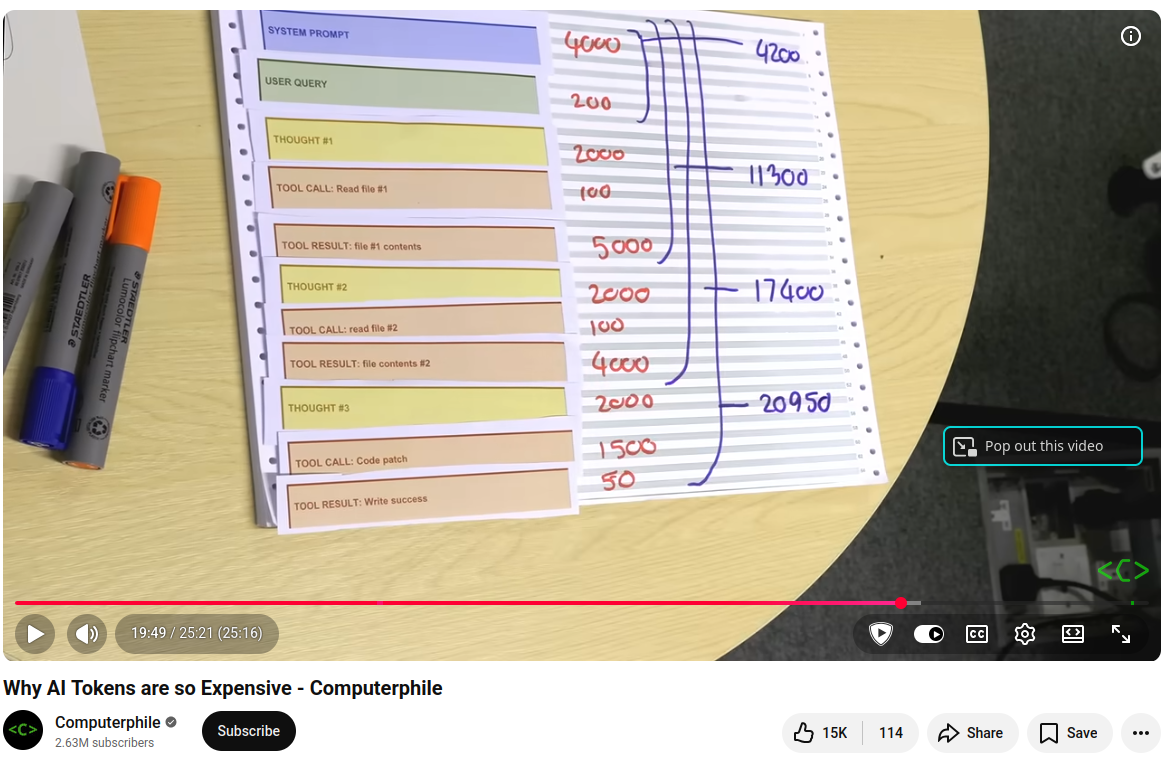
\includegraphics[width=\textwidth]{proprietary-costs.png}
	\end{figure}
\end{frame}

\begin{frame}{Comparing Costs Between Options}
	\begin{exampleblock}{Example: Social Science Experiments}
		\begin{table}[ht]
			\centering
			\begin{tabular}{cccc}
				\toprule
				& CPT & \textbf{Total cost} & \textbf{Infrastructure} \\
				\midrule
				Humans & \$ 9.31 & \$ 16{,}758 & None \\
				GPT-5.1 & \$ 0.25 & \$ 446.32 & None \\
				Local Host& \$ 0.03 & \$ 58.82 & GPU server \\
				Small models & \$ 0.01 & \$ 9.80 & Consumer-grade \\
				\bottomrule
			\end{tabular}
			\caption{\url{https://arxiv.org/abs/2503.16505}}
		\end{table}
	\end{exampleblock}
\end{frame}


\section{Inference Optimization}

\begin{frame}{Outline}
	\tableofcontents[currentsection]
\end{frame}

\subsection{Quantization}

\begin{frame}
	\sectionpage
	\subsectionpage
\end{frame}

% Update this if changed in module 3
\begin{frame}{Reminder: What is Quantization?}
	\begin{columns}
		\begin{column}{0.5\textwidth}
			\begin{figure}
				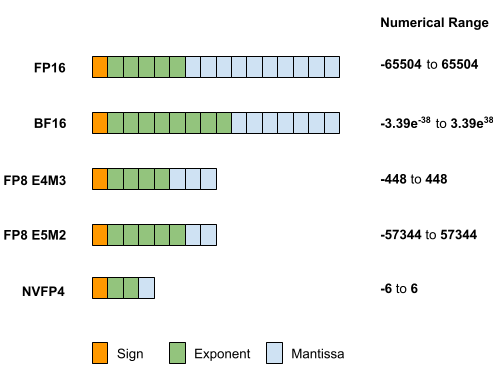
\includegraphics[width=\columnwidth]{quantization-fp.png}
				\centering
				\caption{
					\url{https://developer.nvidia.com/blog/model-quantization-concepts-methods-and-why-it-matters}
				}
			\end{figure}
		\end{column}
		 \begin{column}{0.5\textwidth}
			\only<1>{
				\begin{block}{What is it?}
					\begin{itemize}
						\item Quantization refers to dropping the size (not number)
						of the LLM parameters.
						
						\item Normally, each parameter is stored in a 32 bit
						floating point.
						
						\item Quantization can drop them to usually 4 bits,
						resulting in \alert{$\times 8$ less} GPU memory and
						inference costs.
					\end{itemize}
				\end{block}
				
			}
			\only<2>{
				\begin{block}{Why is it useful?}
					\begin{itemize}
						\item Quantization is one of the \alert{most useful tools}
						at your disposal.
						
						\item Allows for training and inference in consumer-grade
						hardware.
					\end{itemize}
				\end{block}
			}
		\end{column}
	\end{columns}
\end{frame}

\begin{frame}{Floating Point Representations}
	\begin{columns}
		\begin{column}{0.5\textwidth}
			\begin{figure}
				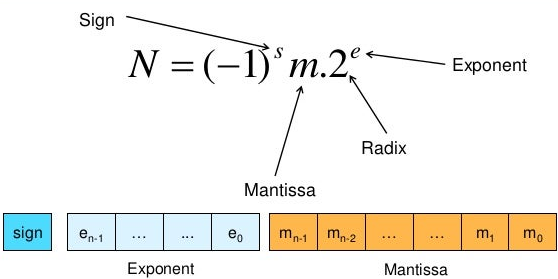
\includegraphics[width=\columnwidth]{floating-point.png}
				\caption{\url{http://www.slideshare.net/DilumBandara/07-data-representation}}
			\end{figure}
		\end{column}
		\begin{column}{0.5\textwidth}
			\begin{itemize}
				\item Real numbers are represented as ``equations'' in computers.
				\item 32 bits.
				\item \textbf{Exponent}: Determines the \alert{range} of possible numbers.
				\item \textbf{Mantissa}: Determines \alert{accuracy}.
			\end{itemize}
		\end{column}
	\end{columns}
\end{frame}

\begin{frame}{FP quantization}
	\begin{columns}
		\begin{column}{0.5\textwidth}
			\begin{figure}
				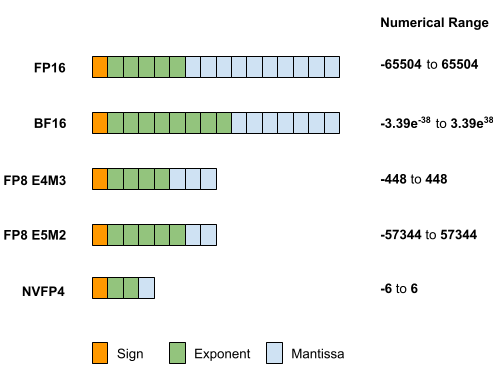
\includegraphics[width=\columnwidth]{quantization-fp.png}
				\caption{\url{http://www.slideshare.net/DilumBandara/07-data-representation}}
			\end{figure}
		\end{column}
		\begin{column}{0.5\textwidth}
			\begin{block}{FP Quantization}
				\begin{itemize}
					\item Works much like rounding numbers.
					\item Simple, intuitive, works well with GPUs.
					\item Many competitive techniques: AWQ, GGUF, GPTQ, ...
				\end{itemize}
			\end{block}
		\end{column}
	\end{columns}
\end{frame}

\begin{frame}{INT quantization}
	\begin{columns}
		\begin{column}{0.5\textwidth}
			\begin{figure}
				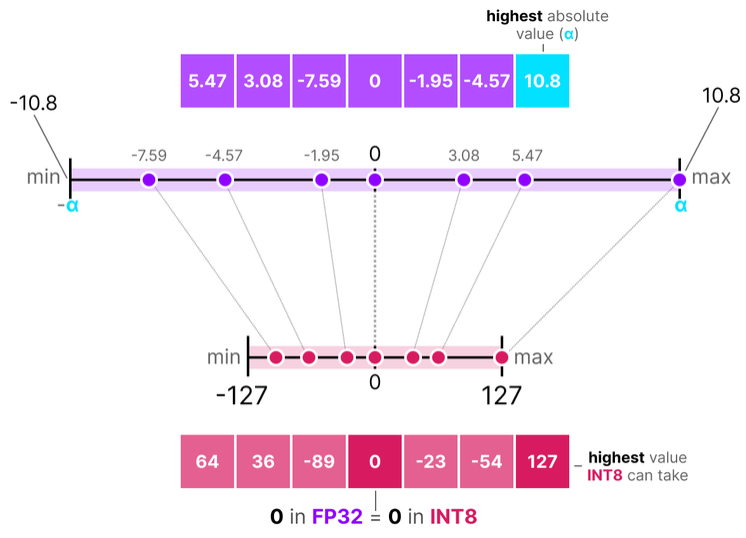
\includegraphics[width=\columnwidth]{quantization-int.png}
				\caption{\url{https://www.maartengrootendorst.com/blog/quantization}}
			\end{figure}
		\end{column}
		\begin{column}{0.5\textwidth}
			\begin{block}{INT Quantization}
				\begin{itemize}
					\item Maps each float to an integer grid.
					\item Two kinds of errors: \textbf{rounding} error (float $\rightarrow$ int), and \textbf{clipping} error (int $\rightarrow$ grid range).\note{Grid range = $x_{min} or x_{max}$}
					\item Extremely efficient with CPUs and specialized hardware.\note{Mention ``fake quantization'' when ran on GPUs}
				\end{itemize}
			\end{block}
		\end{column}
	\end{columns}
\end{frame}

\begin{frame}{Which to Use?}
	\begin{columns}
		\begin{column}{0.5\textwidth}
			\begin{block}{Floating Point}
				\begin{itemize}
					\item Specialized for GPUs.
					\item Well supported.
					\item Smaller errors.
				\end{itemize}	
			\end{block}
		\end{column}
		\begin{column}{0.5\textwidth}
			\begin{block}{Integer}
				\begin{itemize}
					\item Extremely efficient in edge devices and specialized hardware.
					\item Very efficient for CPU inference.
					\item Not supported by GPUs.*
					\item Generally competitive with FP quantization.
				\end{itemize}
			\end{block}
		\end{column}
	\end{columns}
\end{frame}


\subsection{KV Caching}

\begin{frame}
	\sectionpage
	\subsectionpage
\end{frame}

\begin{frame}{What is it?}
	\begin{columns}
		\begin{column}{0.5\textwidth}
			\begin{figure}
				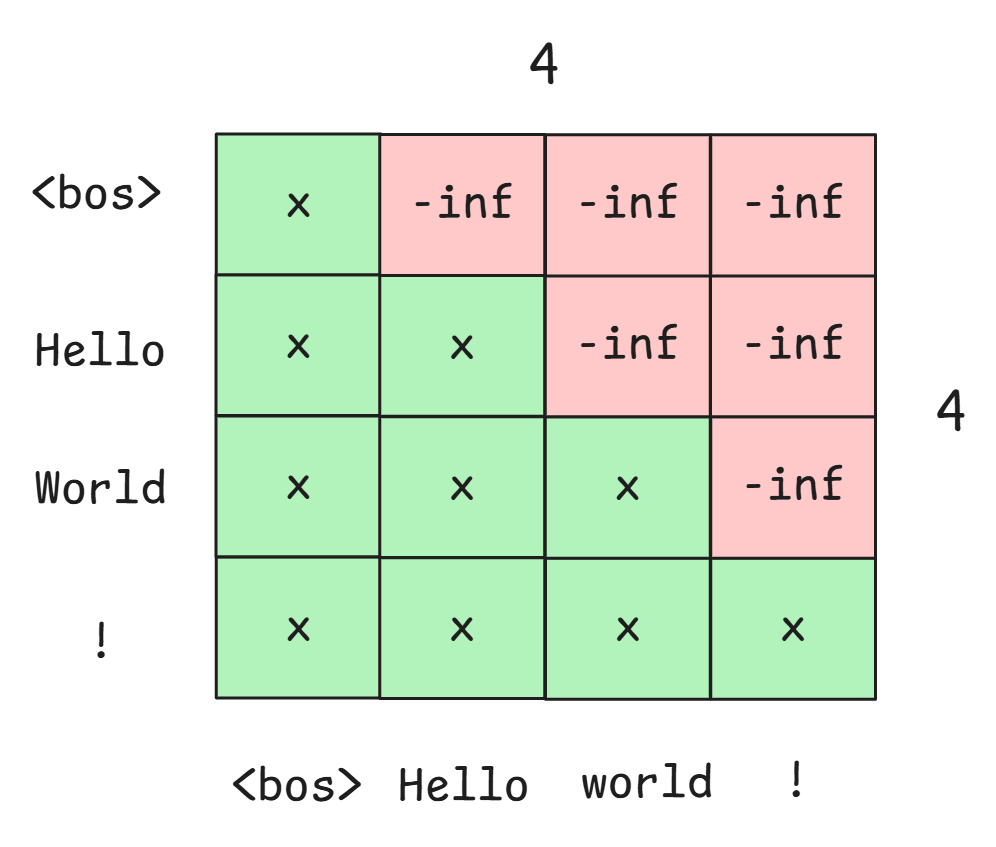
\includegraphics[width=\columnwidth]{kv-cache-example.png}
				\caption{\url{https://huggingface.co/blog/not-lain/kv-caching}}
			\end{figure}	

		\end{column}
		\begin{column}{0.5\textwidth}
			\only<1>{
				\begin{block}{The Problem}
					\begin{itemize}
						\item Transformers are autoregressive.
						\item The more they generate, the harder it gets to generate.
						\item Inference becomes burdened in long contexts.
					\end{itemize}
				\end{block}
			}
			\only<2>{
				\begin{block}{KV Caching}
					\begin{itemize}
						\item KV matrices are the same for all previous steps.
						\item We can simply store them instead of re-computing them.
						\item Thus; a cache for KV matrices!
						\item \alert{Significant} speedup during inference.
						\item \alert{Better} speedup as generation becomes \alert{longer}!
					\end{itemize}
				\end{block}
			}
			\only<3>{
				\begin{block}{KV Caching}
					\begin{itemize}
						\item Cache size stored in GPU.
						\item Scales linearly with context.
						\item $KV cache (bytes) = batch\_size \times context\_length \times 2 \times num\_layers \times num\_kv\_heads \times head\_dim \times bytes\_per\_param$
					\end{itemize}
				\end{block}
			}
		\end{column}
	\end{columns}
\end{frame}

\begin{frame}{Downsides}
	\begin{block}{Formula}
		$KV cache = batch\_size \times context\_length \times 2 \times num\_layers \times num\_kv\_heads \times head\_dim \times bytes\_per\_param$
	\end{block}
	
	\begin{columns}
		\begin{column}{0.5\textwidth}
			\begin{exampleblock}{LLaMa-8B (32K)}
				$KV cache = 1 \times 32,768 \times 2 \times 32 \times 8 \times 128 \times 2
				= 4,294,967,296 bytes
				= 4.0 GB$
			\end{exampleblock}
		\end{column}
		\begin{column}{0.5\textwidth}
			\begin{exampleblock}{LLaMa-8B (128K)}
				$KV cache = 1 \times 131,072 \times 2 \times 32 \times 8 \times 128 \times 2
				= 17,179,869,184 bytes
				= 16.0 GB$
			\end{exampleblock}
		\end{column}
	\end{columns}
	
	\begin{alertblock}{Especially problematic for quantized models.}
		LLaMa-8B 4-bit quantization: $\approx 5GB$.
	\end{alertblock}
\end{frame}


\begin{frame}{Scaling Caches}
	\begin{columns}
		\begin{column}{0.5\textwidth}
			\begin{figure}
				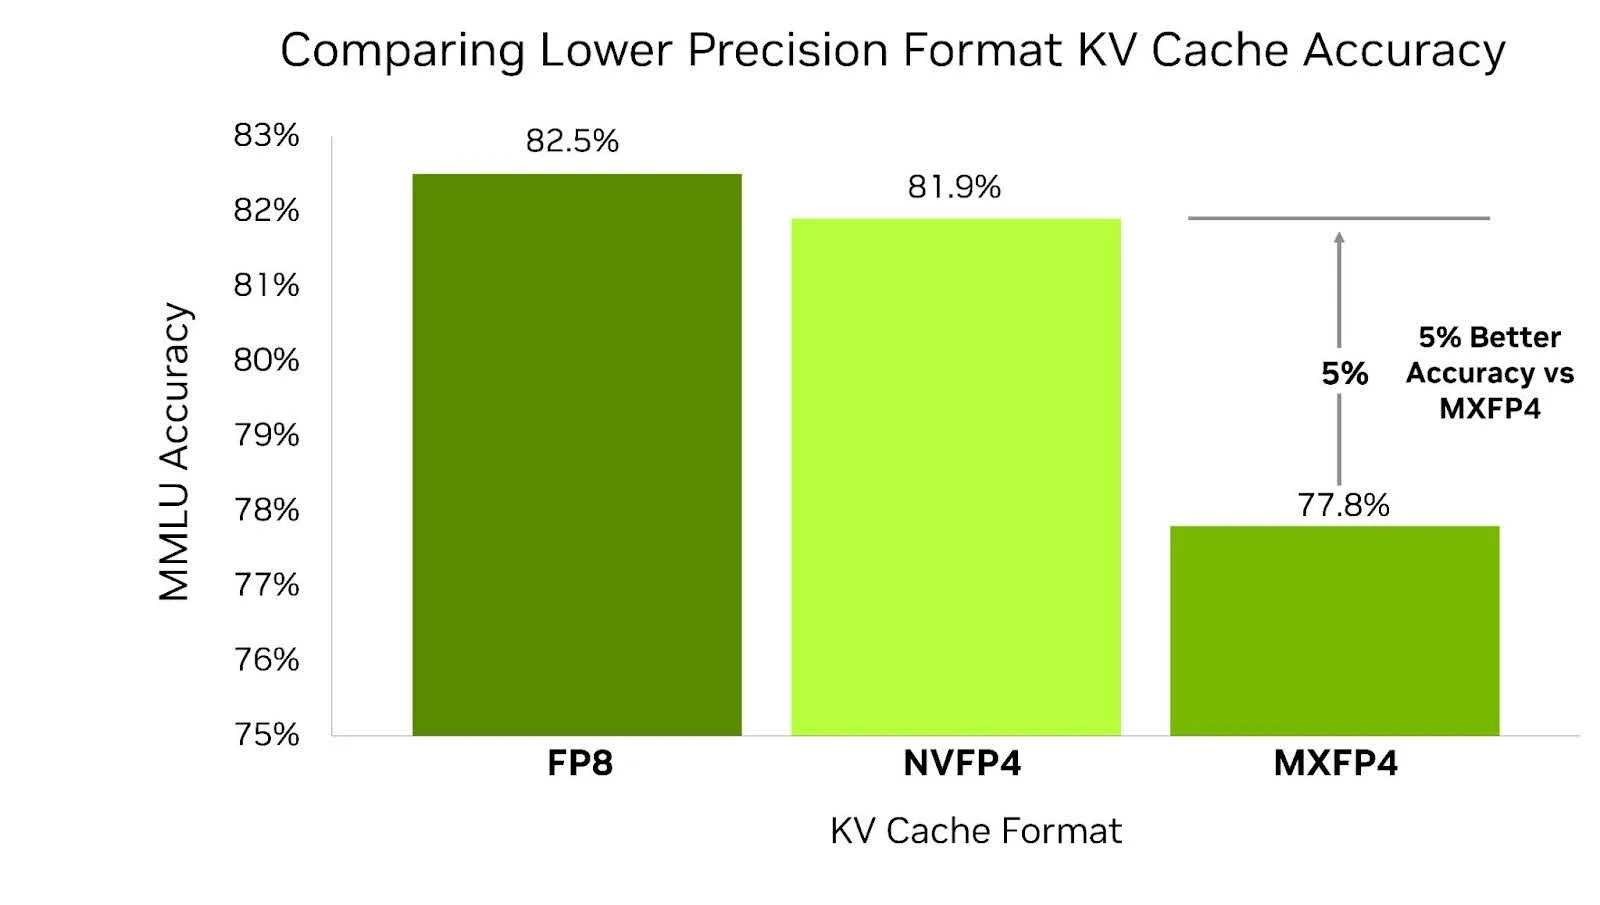
\includegraphics[width=\columnwidth]{kv-cache-quant-size.png}
				\caption{\url{https://developer.nvidia.com/blog/optimizing-inference-for-long-context-and-large-batch-sizes-with-nvfp4-kv-cache}}
			\end{figure}
		\end{column}
		\begin{column}{0.5\textwidth}
			\begin{block}{KV Caching}
				Still in experimental stages.
				\begin{itemize}
					\item Sliding window approach.
					\item Context pruning.
					\item Quantization.
				\end{itemize}
			\end{block}
			
			\begin{alertblock}{But...}
				Perhaps, you don't need all that context in the first place!
			\end{alertblock}
		\end{column}
	\end{columns}
\end{frame}


\section{Evaluation}

\begin{frame}{Outline}
	\tableofcontents[currentsection]
\end{frame}


\subsection{Naive Approaches}

\begin{frame}
	\sectionpage
	\subsectionpage
\end{frame}


\subsection{Quantitative Evaluation}

\begin{frame}
	\sectionpage
	\subsectionpage
\end{frame}


\subsection{HCI Evaluation}

\begin{frame}
	\sectionpage
	\subsectionpage
\end{frame}


\part{Beyond the Money Constraints}

\begin{frame}
	\partpage
\end{frame}

\section{GDPR}

\begin{frame}{Outline}
	\tableofcontents[currentsection]
\end{frame}

\subsection{What is it?}

\begin{frame}
	\sectionpage
	\subsectionpage
\end{frame}

\begin{frame}{GDPR}
		\begin{columns}
		\begin{column}{0.5\textwidth}
			\begin{figure}
				
\includegraphics[width=\columnwidth]{gdpr.jpg}
			\end{figure}
		\end{column}
		\begin{column}{0.5\textwidth}
			\only<1>{
				\begin{block}{General Data Protection Regulation}
					\begin{itemize}
						\item Privacy law concerning almost exclusively \alert{personal data}.
						\item Any information relating to an identified or identifiable natural person (``data subject'').
					\end{itemize}
					\note{From the point of view of the nature of the information, the concept of personal data includes any sort of statements about a person. It covers "objective" information, such as the presence of a certain substance in one's blood. It also includes "subjective" information, opinions or assessments. From the point of view of the content of the information, the concept of personal data includes data providing any sort of information.}
				\end{block}
			}
			\only<2>{
				\begin{block}{Where does it apply?}
					If at least one is true:
					\begin{itemize}
						\item Data subjects are in the Union.
						\item Their behavior takes place in the Union.
						\item Controller or processor in the Union.\note{Due to the previous two, non-EU companies are very frequently subject to GDPR.}
					\end{itemize}
				\end{block}
			}
		\end{column}
	\end{columns}
\end{frame}

\begin{frame}{Identifiable Information}
	\begin{columns}
		\begin{column}{0.5\textwidth}
			\begin{figure}
				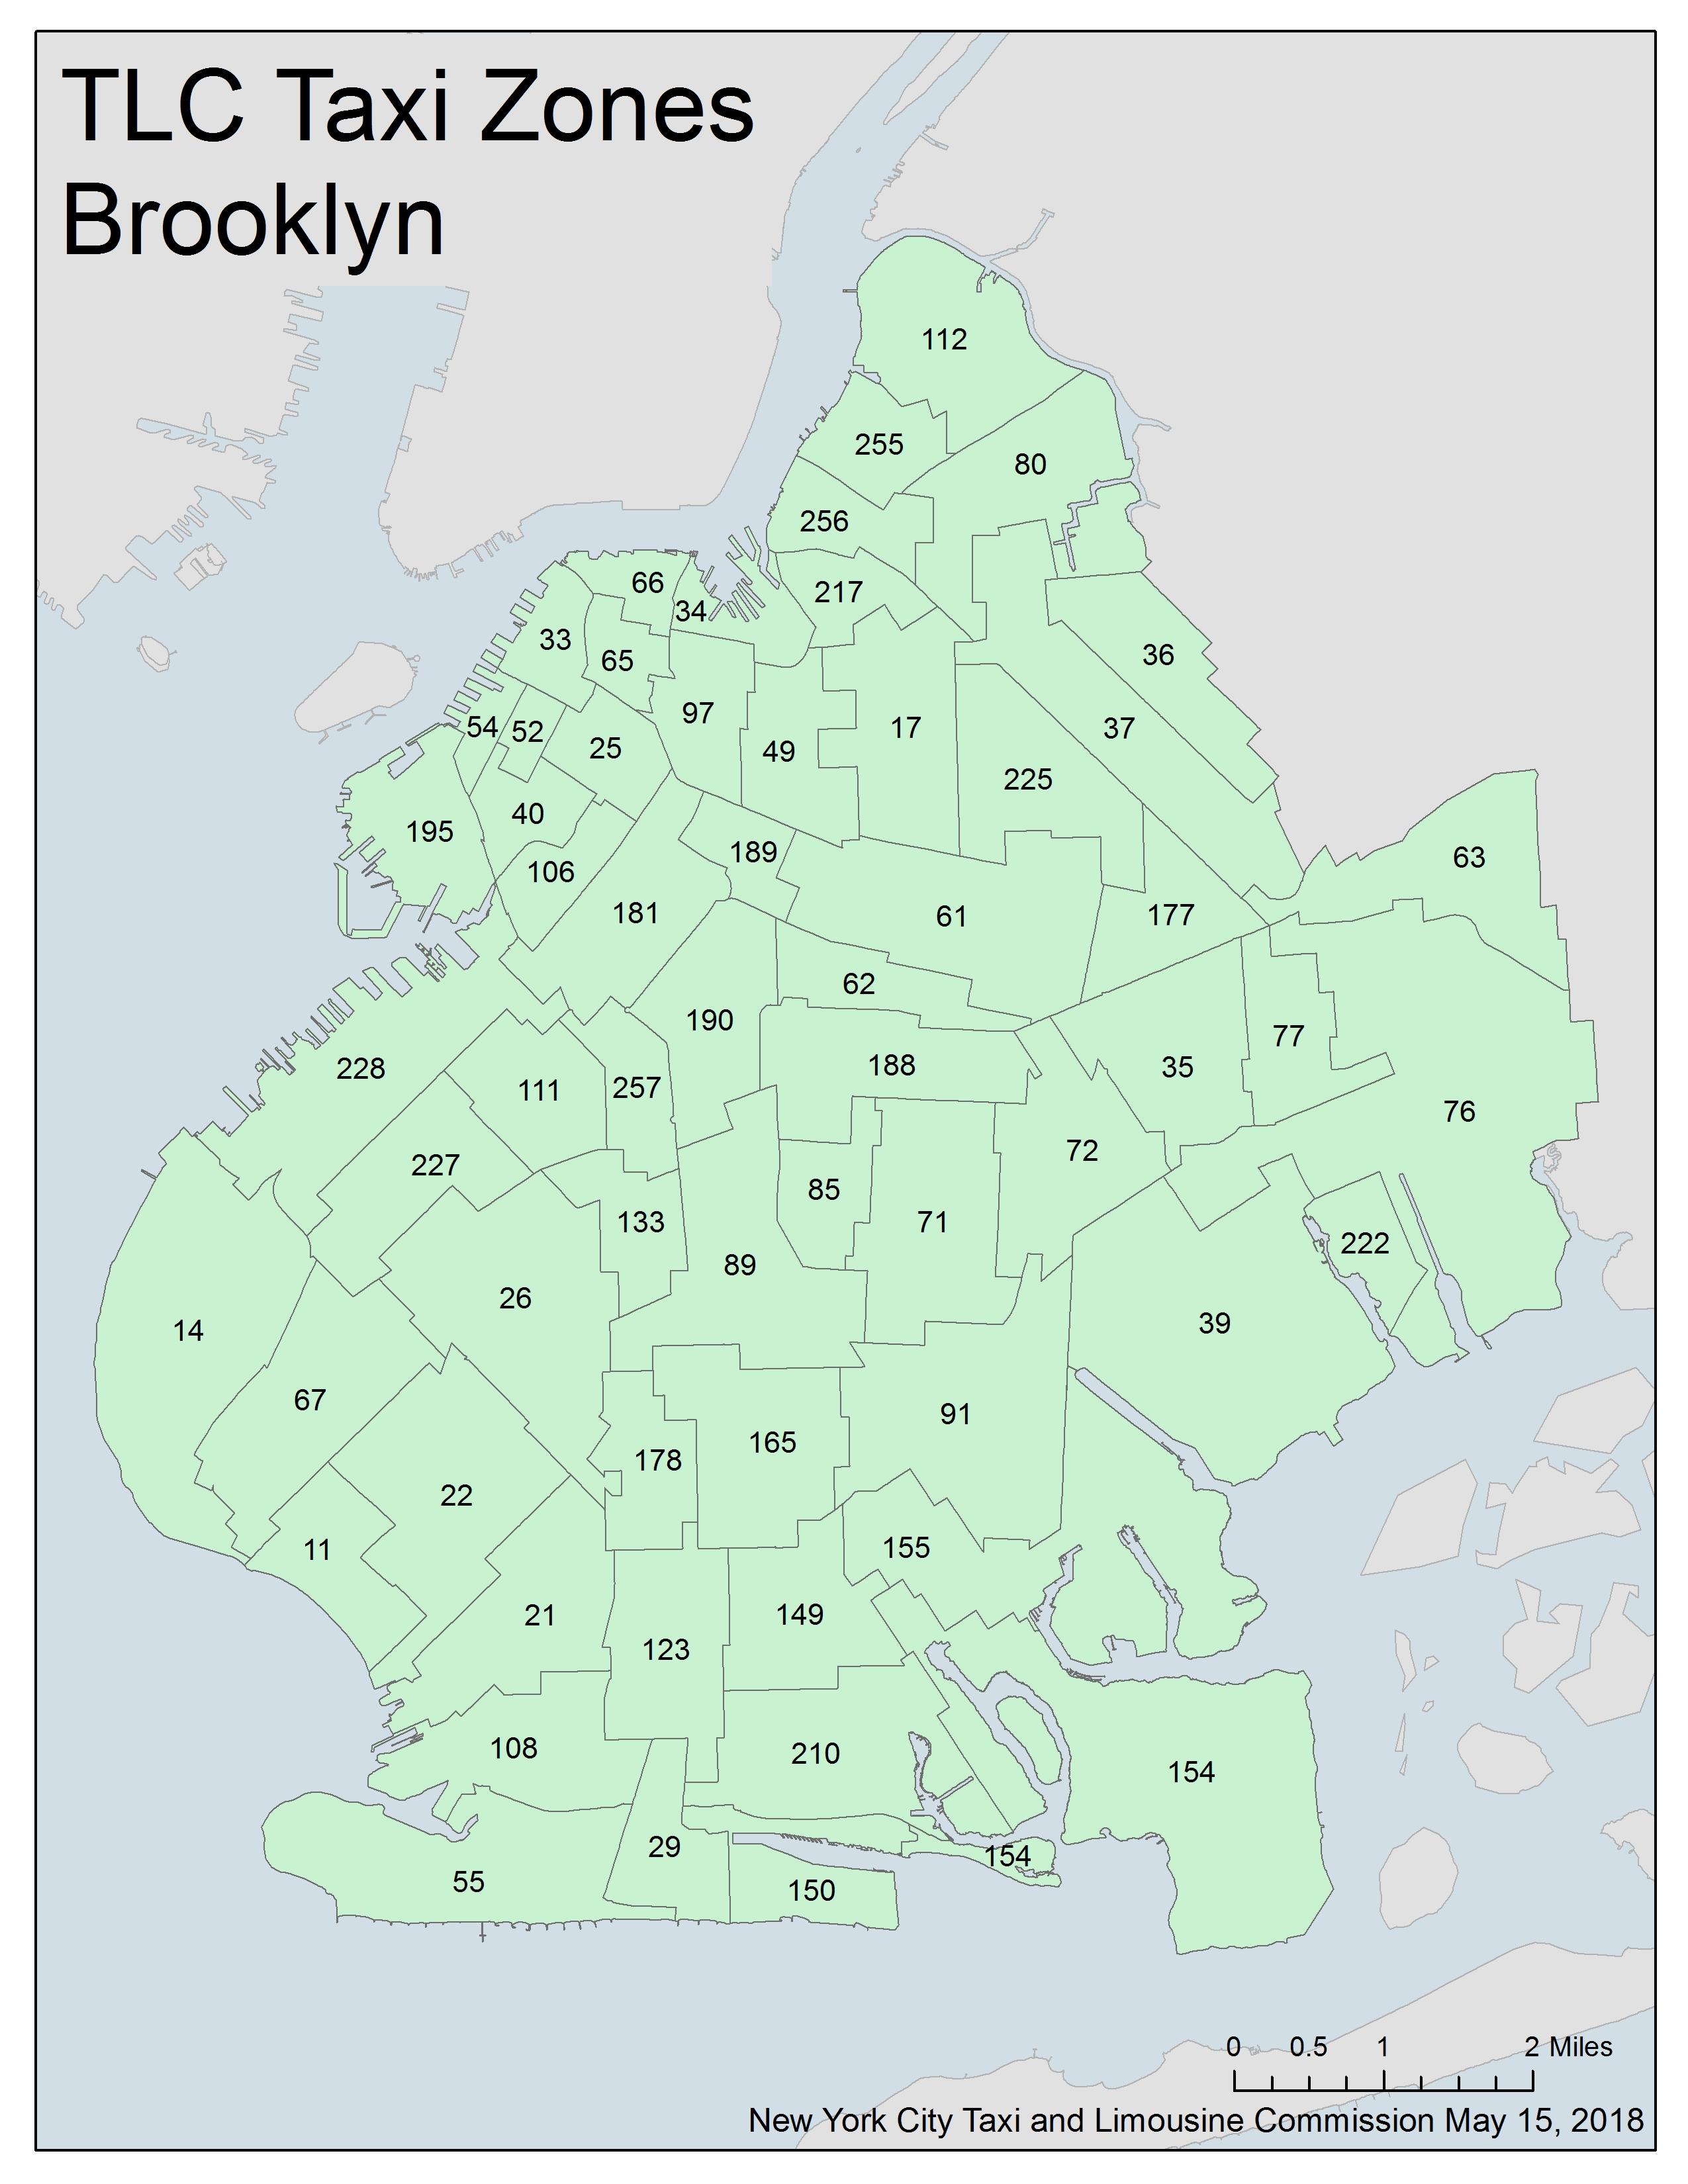
\includegraphics[width=\columnwidth]{nyc-failure-case.jpg}
				\note{NYC Taxi and Limousine Commission (TLC) trip and fare logs: Over 20GB of trip and fare logs from NYC taxis, containing detailed records of trips (pickup/dropoff locations and times) Contained alphanumeric codes for the driver’s license number and taxi medallion number using an MD5 hash. They adhered to highly specific, limited patterns: researchers could calculate the MD5 hash for every single possibility.}
			\end{figure}
		\end{column}
		\begin{column}{0.5\textwidth}
			\begin{block}{Direct Identification}
				Including name, address etc.
			\end{block}
			
			\begin{alertblock}{Indirect Identification}
				\begin{itemize}
					\item Combination of SDB characteristics.
					\item ID number, location.
					\item Hardware/IP address, browser fingerprinting.
				\end{itemize}
			\end{alertblock}
		\end{column}
	\end{columns}
\end{frame}

\begin{frame}{Definitions}
	\begin{columns}
		\begin{column}{0.5\textwidth}
			\begin{block}{Data Controller}
				The natural or legal person, public authority, agency or other body which, alone or jointly with others, \alert{determines the purposes and means} of the processing of personal information.
			\end{block}
		\end{column}
		\begin{column}{0.5\textwidth}
			\begin{block}{Data Processor}
				A natural or legal person, public authority, agency or other body which \alert{processes} personal data \alert{on behalf of the controller}.
			\end{block}
			\pause
			\begin{alertblock}{}
				That's you!
			\end{alertblock}
		\end{column}	
	\end{columns}
\end{frame}


\subsection{Working with GDPR}

\begin{frame}
	\sectionpage
	\subsectionpage
\end{frame}

\begin{frame}{How Should I Comply?}
	\begin{block}{The Seven Principles}
		\only<1>{
			\begin{enumerate}
				\item \textbf{Lawfulness, Fairness, and Transparency}
				
				\item \textbf{Purpose Limitation:} Data must be collected for specified, explicit, and legitimate purposes.
				\note{Any new or incompatible purpose must have a distinct legal basis; disclosure to third parties for a new purpose requires careful consideration and likely an additional legal basis.}
				
				\item \textbf{Data Minimisation/Proportionality:} Data collected must be adequate, relevant, and strictly limited to what is necessary for the declared aim.
				\note{The categories of data chosen must be necessary to achieve the overall aim, and controllers must strictly limit collection to directly relevant information.}
				
				\item \textbf{Accuracy:} Personal data must be accurate and, where necessary, kept up to date.
				\note{Every reasonable step must be taken to ensure that inaccurate data is erased or rectified without delay, mitigating potential damage to the data subject.}
			\end{enumerate}
		}
		\only<2>{
				\begin{enumerate}
					\setcounter{enumi}{4}
					\item \textbf{Storage Limitation:} Data must only be kept in a form that permits identification for no longer than is necessary for the processing purpose.
					\note{An exception applies to archiving, scientific research, or statistical purposes, provided appropriate technical measures are used to safeguard individual rights.}
					
					\item \textbf{Integrity and Confidentiality (Security):} Data must be protected by appropriate technical and organizational measures against unauthorized access, loss, or damage.
					\note{This principle serves as the key mechanism for preventing adverse effects for the data subject during data processing.}
					
					\item \textbf{Accountability:} Controllers must actively implement and continuously demonstrate compliance with all data protection provisions in their activities.
					\note{The controller is responsible for demonstrating compliance to data subjects, the public, and supervisory authorities at any time (e.g., keeping records, conducting impact assessments).}
				\end{enumerate}
		}
	\end{block}
\end{frame}

\begin{frame}{How Should I Comply?}
	\begin{block}{Data protection by design/by default}
		\begin{itemize}
			\item Design your data collection and analysis \alert{proactively}.
			\item Maximum privacy is the default. Users can opt out.
			\item Keep users informed. Keep the system user-centric.
			\item Keeping \alert{minimal personal data} $\rightleftarrows$ minimum risk and complications.
		\end{itemize}
	\end{block}
	
	\begin{block}{Data Protection Officer (DPO)}
		Data Controllers are typically required to have a \alert{designated expert} trained on this legislation.
	\end{block}
\end{frame}

\begin{frame}{How Far Should I Go?}
	\begin{alertblock}{High-risk systems}
		\begin{itemize}
			\item Evaluation or scoring, including profiling and predicting
			\item Automated-decision making with legal or similar significant effect
			\item Datasets that have been matched or combined
			\item Data concerning vulnerable data subjects
		\end{itemize}
	\end{alertblock}
\end{frame}

\begin{frame}{How do I Remove Personal Information?}
	\begin{block}{Common Methods}
		\begin{itemize}
			\item Collect data without personal information (Data minimization principle).
			\item Anonymize: All identifying elements are eliminated from a set of personal data so that the data subject is no longer identifiable.
			\item Redaction/Expungement: ``Right to be forgotten''.
		\end{itemize}
	\end{block}
\end{frame}

\begin{frame}{How do I Remove Personal Information?}
	\begin{columns}
		\begin{column}{0.5\textwidth}
			\begin{figure}
				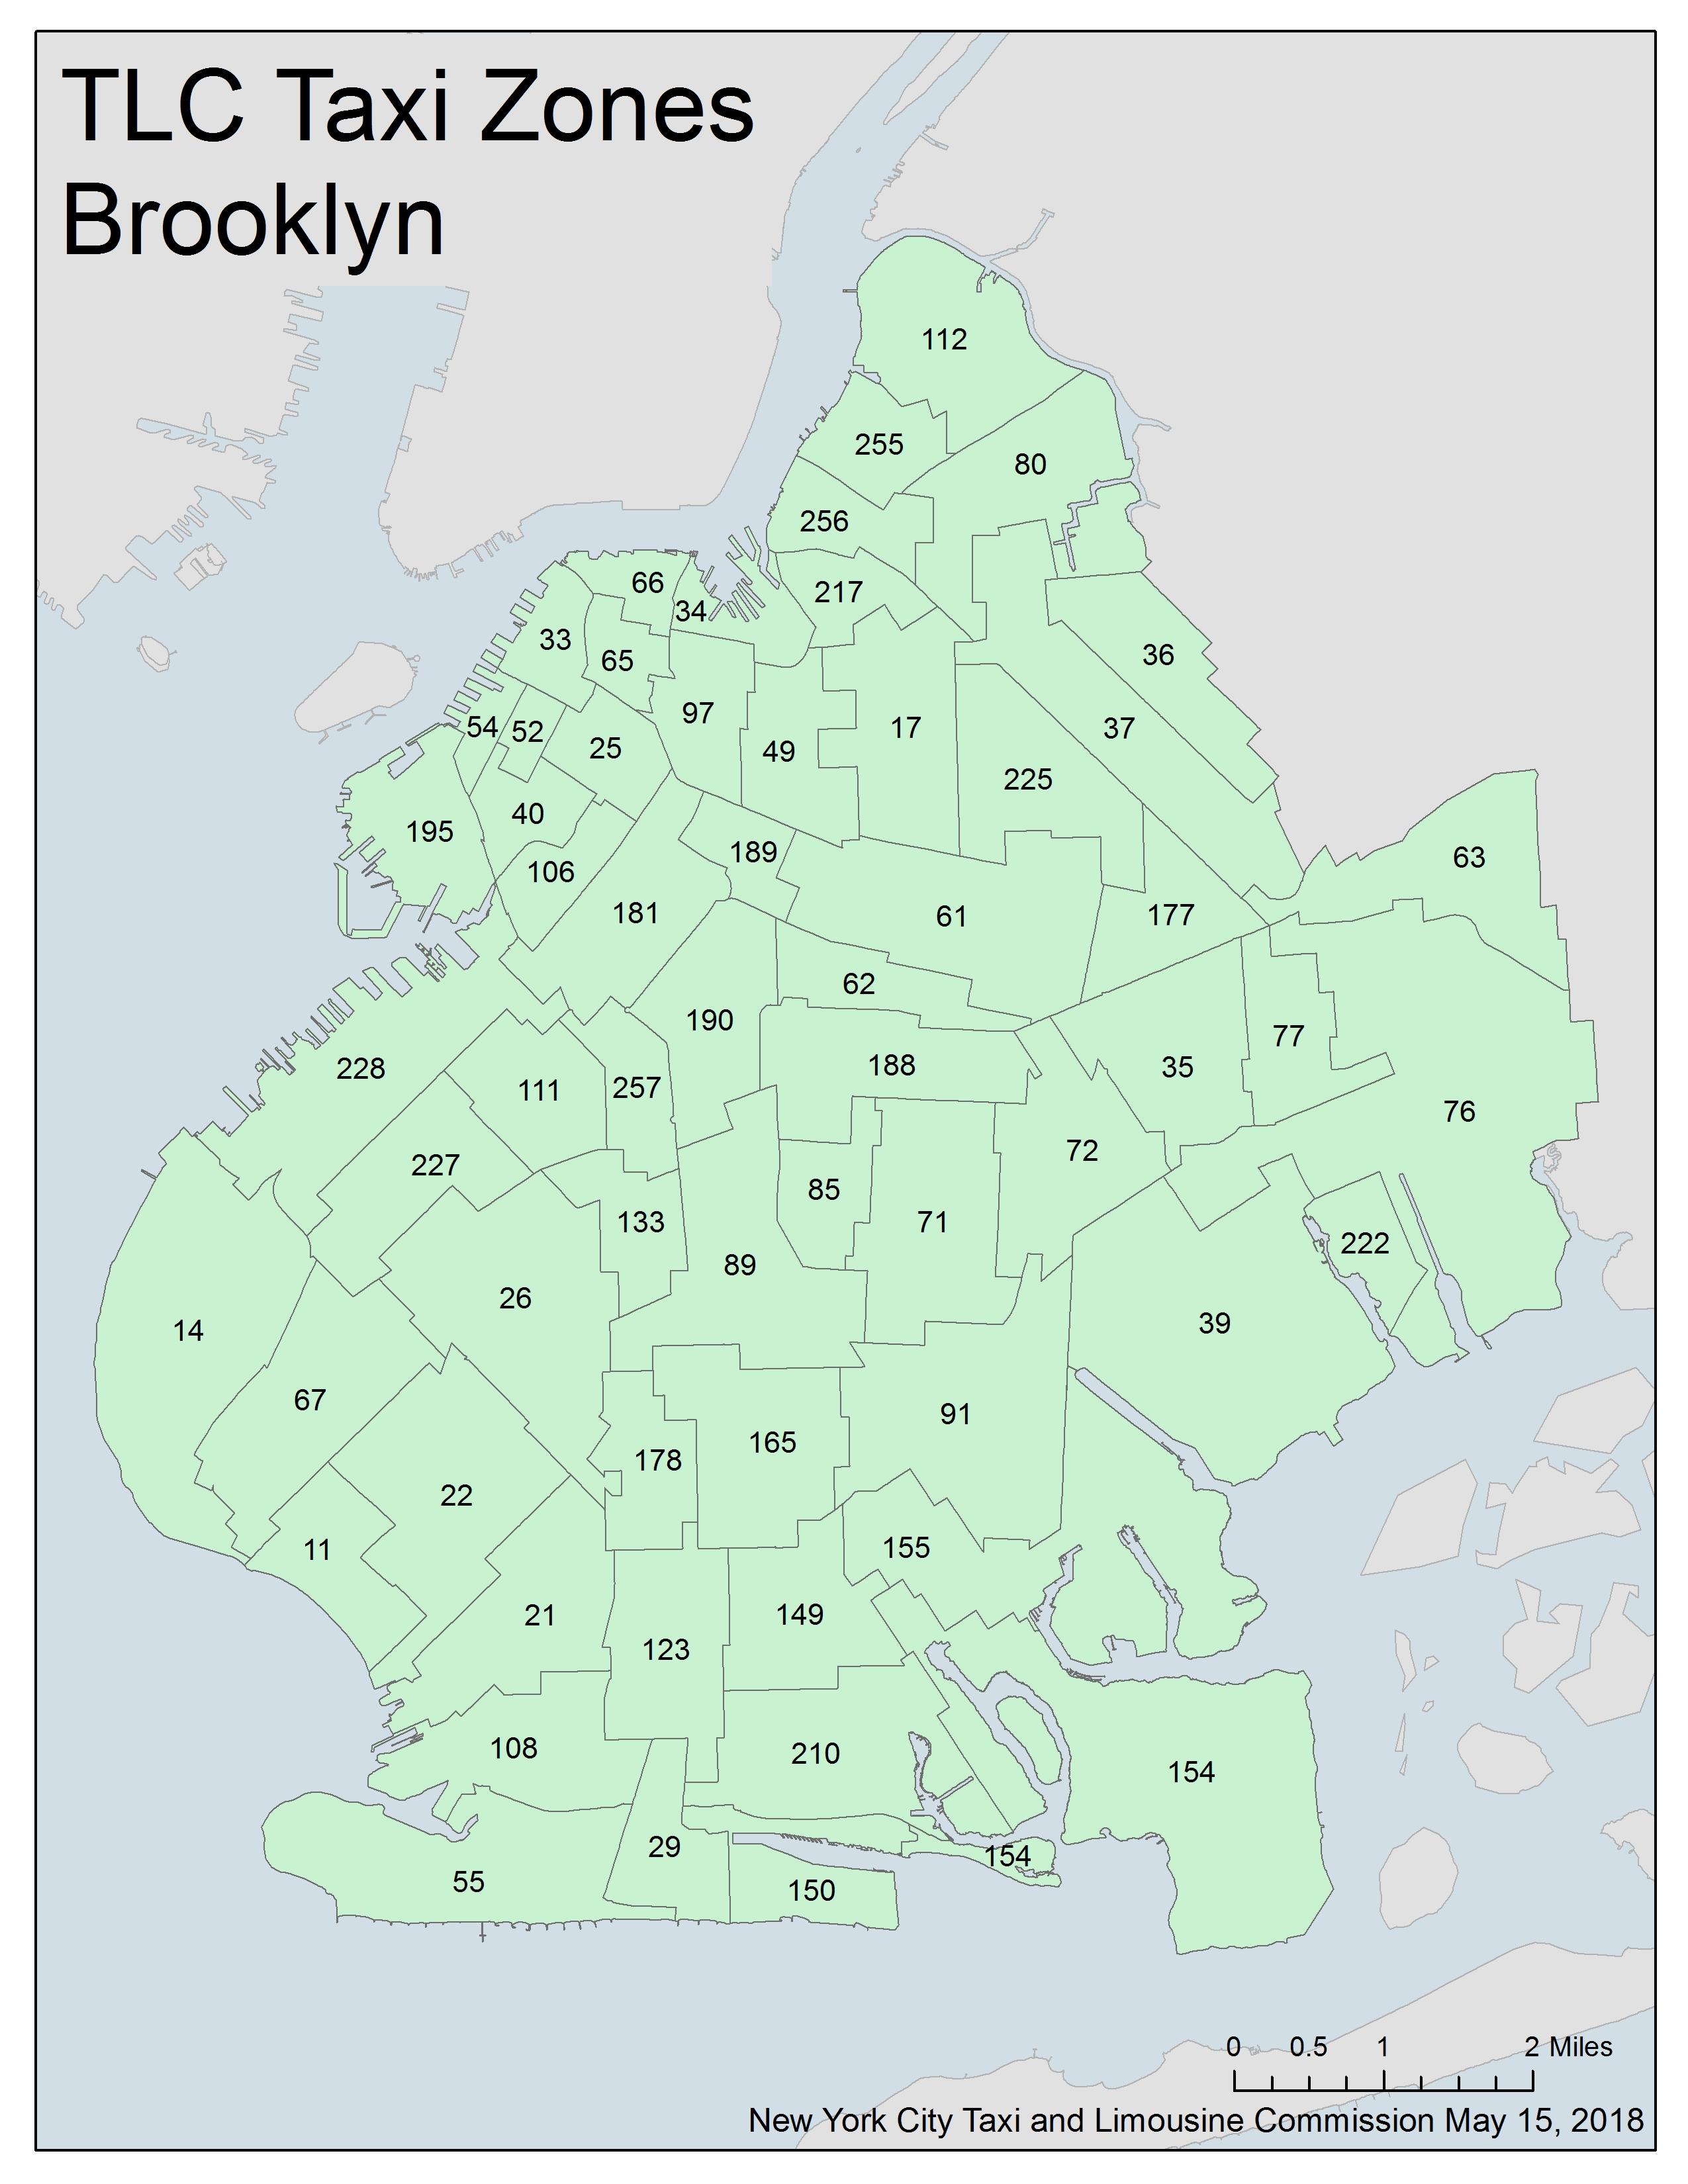
\includegraphics[width=\columnwidth]{nyc-failure-case.jpg}
				\note{NYC Taxi and Limousine Commission (TLC) trip and fare logs: Over 20GB of trip and fare logs from NYC taxis, containing detailed records of trips (pickup/dropoff locations and times) Contained alphanumeric codes for the driver’s license number and taxi medallion number using an MD5 hash. They adhered to highly specific, limited patterns: researchers could calculate the MD5 hash for every single possibility.}
			\end{figure}
		\end{column}
		
		\begin{column}{0.5\textwidth}
			\begin{alertblock}{Pseudo-anonymization is not enough}
					Attributes, such as name, date of birth, sex, address, or other elements that could lead to identification are replaced by a pseudonym.
			\end{alertblock}
		\end{column}
	\end{columns}
\end{frame}


\section{EU AI Act}

\begin{frame}{Outline}
	\tableofcontents[currentsection]
\end{frame}

\subsection{What is it?}

\begin{frame}
	\sectionpage
	\subsectionpage
\end{frame}

\begin{frame}{EU AIA}
	\begin{columns}
		\begin{column}{0.5\textwidth}
			\begin{figure}
				
\includegraphics[width=\columnwidth]{ai_act.jpg}
			\end{figure}
		\end{column}
		\begin{column}{0.5\textwidth}
			\begin{block}{Purpose}
				\begin{itemize}
					\item Supplementary to other legislation (e.g., GDPR).
					\item Applicable to all AI systems in the Union.
					\item Classify systems by internal risk, restrict them appropriately.
				\end{itemize}
			\end{block}
		\end{column}
	\end{columns}
\end{frame}

\begin{frame}{Scope}
	\begin{columns}
		\begin{column}{0.5\textwidth}
			\begin{figure}
				
\includegraphics[width=\columnwidth]{ai_act.jpg}
			\end{figure}
		\end{column}
		\begin{column}{0.5\textwidth}
			\only<1>{
				\begin{block}{Where does it apply?}
					\begin{itemize}
						\item \alert{Providers} placing AI systems in the Union.\note{Includes non-Union providers.}
						\item \alert{Users} of AI systems in the Union.
						\item Importers, distributors, manufacturers, representatives and affected persons using or operating systems whose \alert{outputs} are used within the Union.\note{Deployer: uses an AI system. Authorized representative: EU entity which has received and accepted a written mandate from a provider or developer to carry out tasks and obligations on their behalf.}
					\end{itemize}
				\end{block}
			}
			\only<2>{
				\begin{block}{Where does it NOT apply?}
					\begin{itemize}
						\item National security \& defense.
						\item Research / RnD (excluding live testing).
						\item Purely personal activities.
					\end{itemize}
				\end{block}
			}
		\end{column}
	\end{columns}
\end{frame}

\begin{frame}{What is an AI System?}
	\begin{definition}[AI System]
		\begin{itemize}
			\item A \alert{machine}-based system.\note{Hardware and software, enables model training, data processing, predictive modeling, or automated decision-making at scale.}
			\item Operate with varying levels of \alert{autonomy}.\note{Which we will talk about in later slides.}
			\item \alert{Infers} how to generate outputs from input.\note{Includes logic- and knowledge-base approaches.}
			\item (Optional) Adaptive after deployment
		\end{itemize}		
	\end{definition}
\end{frame}

\subsection{Working with the EU AIA}

\begin{frame}
	\sectionpage
	\subsectionpage
\end{frame}

\begin{frame}{Restrictions}
	\begin{figure}
		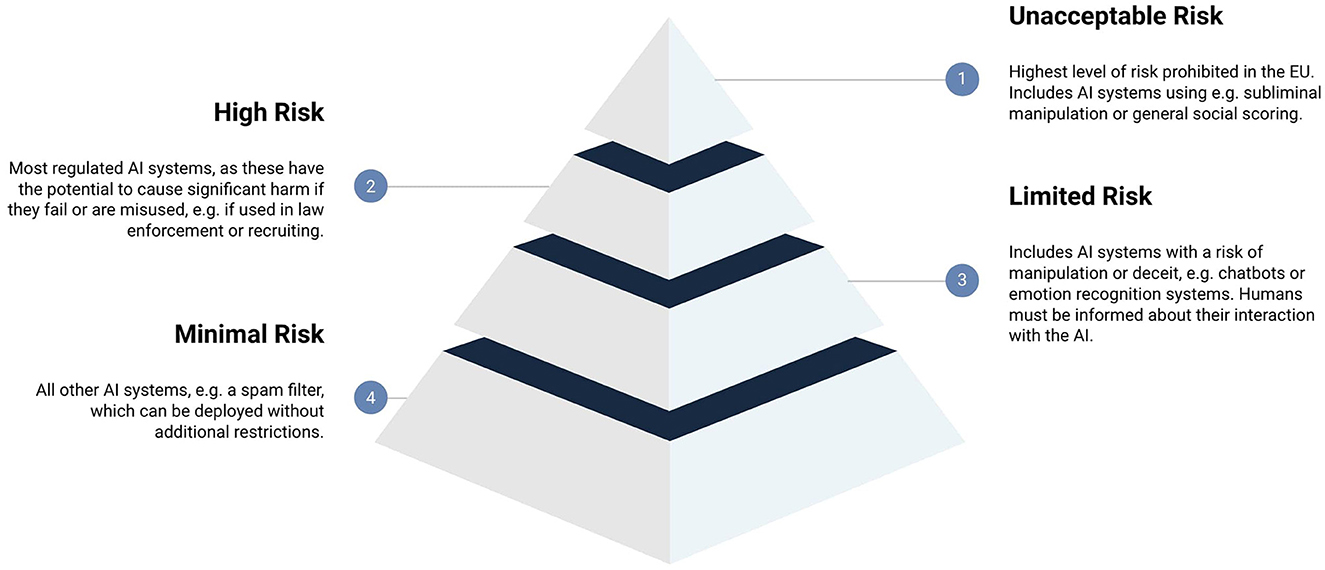
\includegraphics[width=\textwidth]{ai_act_risk.jpg}
		\caption{Image by \url{https://www.frontiersin.org/journals/political-science/articles/10.3389/fpos.2024.1451601/full}, released under CC.}
	\end{figure}
\end{frame}

\begin{frame}{Restrictions: Unacceptable Risk}
	\begin{columns}
		\begin{column}{0.5\textwidth}
			\begin{figure}
				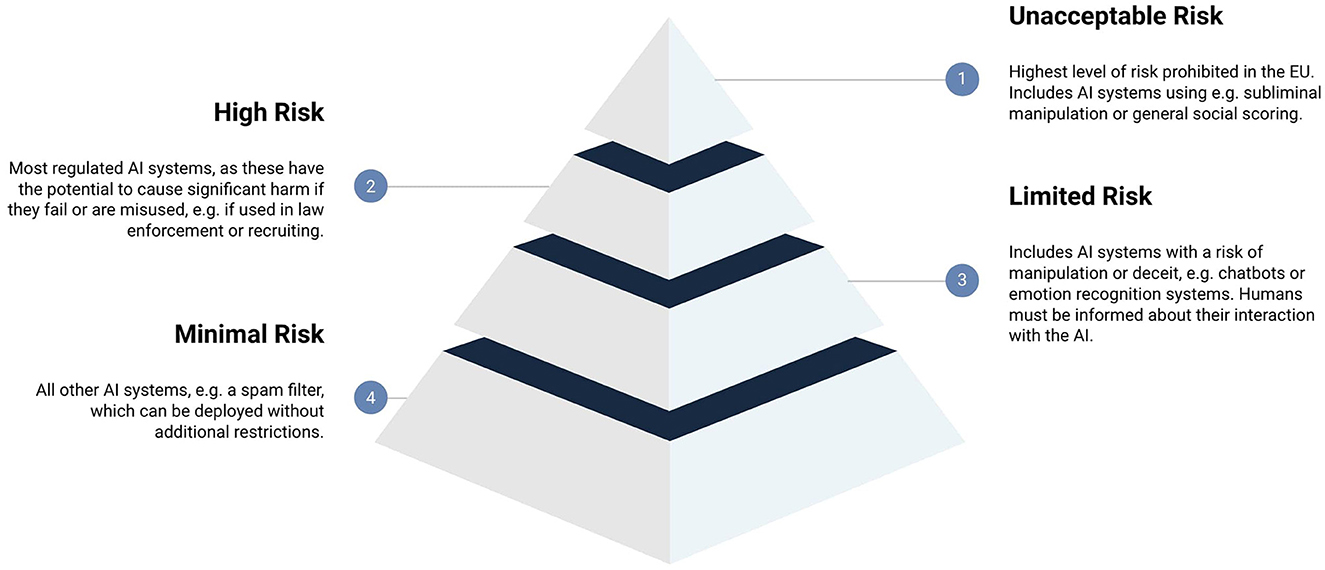
\includegraphics[width=\columnwidth]{ai_act_risk.jpg}
				\caption{Image by \url{https://www.frontiersin.org/journals/political-science/articles/10.3389/fpos.2024.1451601/full}, released under CC.}
			\end{figure}
		\end{column}
		\begin{column}{0.5\textwidth}
			\only<1>{
				\begin{alertblock}{Unacceptable Risk}
					\begin{itemize}
						\item System directly violates core EU principals. 
						\item \alert{Prohibited}.
						\item Example: Emotion recognition in the workplace, unless for medical or safety reasons\note{e.g., tiredness levels of a pilot};
					\end{itemize}
				\end{alertblock}
			}
			\only<2>{
				\begin{block}{High Risk}
					\begin{itemize}
						\item Failure may endanger health and safety. 
						\item Examples: Critical infrastructure, hiring, essential services. 
						\item Requires development of a \alert{risk management system}.
					\end{itemize}
				\end{block}
			}
		\end{column}
	\end{columns}
\end{frame}

\begin{frame}{Restrictions: High Risk}
	\begin{block}{A high-risk system must include:}
		\begin{itemize}
			\item A Risk Management System.\note{Identify misuse, risks, take measures, post-marketing monitoring.}
			\item Data Governance.\note{Besides privacy, formulate assumptions on what the data represents.}
			\item Technical documentation.
			\item Logging system.
			\item Transparency for human users.
			\item Human oversight.\note{e.g., human UI, proportional to risks}
			\item Minimum information use.
			\item Ensure accuracy, robustness.\note{Coordination with EU Commission.}
		\end{itemize}
	\end{block}
\end{frame}
	
	
\section{OpSec}

\begin{frame}{Outline}
	\tableofcontents[currentsection]
\end{frame}

\begin{frame}{What is it?}
	\begin{definition}[OpSec]
		NIST SP 800-53: A process by which potential adversaries can be denied information about capabilities and intentions[...].
	\end{definition}
	\pause
	\begin{alertblock}{}
		Information that your institution wants to keep secret.
	\end{alertblock}
\end{frame}

\begin{frame}{Why do we care?}
	\begin{alertblock}{If you are working with:}
		\begin{itemize}
			\item Personal data.
			\item Medical or otherwise sensitive data.
			\item Internal data (such as customer details).
		\end{itemize}
		Then it is \alert{crucial} that these data remain in your institution.\note{Throwback to GDPR}
	\end{alertblock}
	
	\begin{block}{Applies both if:}
		\begin{itemize}
			\item Your system uses LLM agents.
			\item You yourself use LLM agents.
		\end{itemize}
	\end{block}
\end{frame}

\begin{frame}{Proprietary models}
	\begin{columns}
		\begin{column}{0.5\textwidth}
			\begin{figure}
				
\includegraphics[width=0.45\columnwidth]{claude.jpg}
				
\includegraphics[width=0.45\columnwidth]{openai.png}
				
\includegraphics[width=0.45\columnwidth]{gemini.png}
			\end{figure}
		\end{column}
		\begin{column}{0.5\textwidth}
			\begin{block}{}
				\begin{itemize}
					\item Many providers explicitly state that input data can be used for further model pretraining.
					\item There is no guarantee that API-based models respect user agreements on safeguarding input.
					\item See: Benchmark leakage.
				\end{itemize}
			\end{block}
		\end{column}
	\end{columns}
\end{frame}

\begin{frame}{Solutions}
	\begin{block}{}
		No agreed-upon strategy.
		\begin{itemize}
			\item Identify attack surface. Which data do we need to keep private?
			\item Anonymization.\note{Does not work on all data e.g., business strategies.}
			\item Use locally hosted models for sensitive tasks.\note{Also cheaper! See: quantization}
		\end{itemize}
	\end{block}
\end{frame}

\end{document}
